% =====================================================================================
% FlowState --- Paper 3 of the Trivijaya Quant Research programme.
%
% NO NUMBER IS TYPED INTO THIS FILE. Every quantitative claim resolves through a macro
% defined in flowstate_numbers.tex, generated by scripts/build_flowstate_numbers.py from the
% frozen artifacts. scripts/check_paper_numbers.py fails the build if a bare numeral appears
% in a claim position, and tests/eval/test_numbers.py proves that gate can fail.
%
% Compile: pdflatex flowstate && pdflatex flowstate   (twice, for the contents)
% =====================================================================================
\documentclass[11pt,a4paper]{article}

\newcommand{\paperName}{FlowState}
\newcommand{\paperSubtitle}{A strategy is real and robust.\\ How much money can it take?}
\newcommand{\paperNumber}{3}
\newcommand{\paperShortHead}{Robustness $\rightarrow$ scale}

% =====================================================================================
% Shared style for the three papers of the Trivijaya Quant Research programme.
%
% The three papers report one programme and must look like it: same typography, same
% heading hierarchy, same table rules, same panel vocabulary, same cover structure.
% Anything paper-specific (title, running head, abstract) stays in the paper's own file.
%
% Each paper defines, BEFORE inputting this file:
%   \paperName        e.g. AlphaAudit
%   \paperSubtitle    the one-line question the paper answers
%   \paperNumber      1, 2 or 3
%   \paperShortHead   the right-hand running head
% =====================================================================================

\usepackage[utf8]{inputenc}
\usepackage[T1]{fontenc}
\usepackage{lmodern}
\usepackage[scaled=0.92]{helvet}          % sans face, headings only
\usepackage[margin=1.05in,top=1.15in,bottom=1.1in]{geometry}
\usepackage{microtype}
\usepackage{amsmath,amssymb}
\usepackage{booktabs}
\usepackage{array}
\usepackage{graphicx}
\usepackage{xcolor}
\usepackage[most]{tcolorbox}
\usepackage{titlesec}
\usepackage{enumitem}
\usepackage[font=small,labelfont={bf,color=navy},labelsep=period]{caption}
\usepackage{fancyhdr}
\usepackage{natbib}
\usepackage[colorlinks=true]{hyperref}   % loaded last, as hyperref requires

% The rupee sign is not in the default T1 encoding. A plain "Rs." is unambiguous, renders
% identically on every machine, and avoids a font dependency a reader would have to satisfy
% before they could compile the paper that asks them to check our numbers.
\providecommand{\rupee}{\textrm{Rs.}\,}

% ---- Palette: white ground, blues, one warm accent for our own errors ---------------
\definecolor{navy}{HTML}{0E2E5C}
\definecolor{steel}{HTML}{2C6BA8}
\definecolor{sky}{HTML}{5B93C7}
\definecolor{mist}{HTML}{F0F5FB}
\definecolor{ash}{HTML}{F6F7F9}
\definecolor{ink}{HTML}{1A1A1A}
\definecolor{rust}{HTML}{9C4221}

\color{ink}
\hypersetup{linkcolor=steel, citecolor=steel, urlcolor=steel}

% ---- Repository, cited often enough to deserve one definition ----------------------
\newcommand{\repourl}{https://github.com/Ashwin-aadi/Trivijaya-Quant-Research}
\newcommand{\repo}{\href{\repourl}{\texttt{github.com/Ashwin-aadi/Trivijaya-Quant-Research}}}
\newcommand{\siteurl}{https://ashwin-aadi.github.io/Trivijaya-Quant-Research/}
\newcommand{\site}{\href{\siteurl}{\texttt{ashwin-aadi.github.io/Trivijaya-Quant-Research}}}

% ---- Headings ----------------------------------------------------------------------
\newcommand{\sectionrule}{{\color{sky}\rule{\linewidth}{0.5pt}}\vspace{-0.9em}}
\titleformat{\section}[block]
  {\sffamily\large\bfseries\color{navy}}
  {\colorbox{navy}{\textcolor{white}{\sffamily\bfseries\ \thesection\ }}}{0.7em}{}
  [\vspace{0.25em}\sectionrule]
\titleformat{\subsection}[block]
  {\sffamily\normalsize\bfseries\color{navy}}{\thesubsection}{0.6em}{}
\titleformat{\paragraph}[runin]
  {\sffamily\bfseries\color{navy}}{}{0em}{}[\;]
\titlespacing*{\section}{0pt}{1.6em}{0.8em}
\titlespacing*{\subsection}{0pt}{1.2em}{0.5em}

% ---- Running head ------------------------------------------------------------------
\pagestyle{fancy}\fancyhf{}
\renewcommand{\headrulewidth}{0.4pt}
\renewcommand{\headrule}{{\color{sky}\hrule height 0.4pt}}
\fancyhead[L]{\sffamily\scriptsize\color{navy}\MakeUppercase{\paperName}}
\fancyhead[R]{\sffamily\scriptsize\color{navy}\paperShortHead}
\fancyfoot[C]{\sffamily\scriptsize\color{navy}\thepage}
\fancypagestyle{plain}{\fancyhf{}\renewcommand{\headrulewidth}{0pt}
  \fancyfoot[C]{\sffamily\scriptsize\color{navy}\thepage}}

% ---- Panels ------------------------------------------------------------------------
% A finding the reader must not skim past.
\newtcolorbox{finding}[1][]{
  enhanced, breakable, colback=mist, colframe=steel, boxrule=0pt,
  leftrule=2.5pt, arc=1pt, left=9pt, right=9pt, top=7pt, bottom=7pt,
  coltext=navy, fonttitle=\sffamily\bfseries\small, #1}

% A place where we report our own error. Deliberately a different colour from the findings,
% so a reader flipping through can see at a glance that the paper contains both.
\newtcolorbox{selfreport}[1][]{
  enhanced, breakable, colback=ash, colframe=rust, boxrule=0pt,
  leftrule=2.5pt, arc=1pt, left=9pt, right=9pt, top=7pt, bottom=7pt,
  fonttitle=\sffamily\bfseries\small, #1}

% What a result does *not* license. Every headline in this programme has one of these, because
% the distance between "we measured X on our corpus" and "X is true of AI" is where this
% literature goes wrong.
\newtcolorbox{scopebox}[1][]{
  enhanced, breakable, colback=white, colframe=sky, boxrule=0.6pt,
  arc=1pt, left=9pt, right=9pt, top=6pt, bottom=6pt,
  fonttitle=\sffamily\bfseries\small, title={\sffamily\bfseries What this does not say}, #1}

\newcommand{\keyfinding}[1]{\begin{finding}#1\end{finding}}

% A one-line takeaway that sits directly against a figure or table.
\newcommand{\takeaway}[1]{%
  \vspace{-0.4em}\noindent{\small\sffamily\color{navy}\textbf{Takeaway.}\ #1}\vspace{0.5em}}

% ---- Tables ------------------------------------------------------------------------
\newcommand{\thead}[1]{{\sffamily\bfseries\color{navy}#1}}
\renewcommand{\arraystretch}{1.15}

\setlist[itemize]{leftmargin=1.3em, itemsep=0.25em, topsep=0.4em}
\setlist[enumerate]{leftmargin=1.6em, itemsep=0.35em, topsep=0.4em}

% ---- Evidence-scope tags -----------------------------------------------------------
% The programme's central discipline: every finding is tagged with the population it was
% measured on, so a local-corpus observation can never be read as a statement about AI.
\newcommand{\tagbox}[2]{{\sffamily\scriptsize\textbf{\textcolor{#1}{[#2]}}}}
\newcommand{\taglocal}{\tagbox{steel}{LOCAL 7B}}
\newcommand{\tagfrontier}{\tagbox{navy}{FRONTIER}}
\newcommand{\tagmethod}{\tagbox{navy}{GENERATION METHOD}}
\newcommand{\tagindep}{\tagbox{rust}{GENERATOR-INDEPENDENT}}
\newcommand{\tagexpl}{\tagbox{rust}{EXPLORATORY}}
\newcommand{\tagprereg}{\tagbox{steel}{PRE-REGISTERED}}

% ---- Cover page --------------------------------------------------------------------
\newcommand{\programmecover}[1]{%
\begin{titlepage}
\thispagestyle{empty}
\raggedright
\vspace*{0.6in}
{\sffamily\small\color{steel}\MakeUppercase{Trivijaya Quant Research Programme}\\[0.2em]
 \color{sky}\rule{\linewidth}{1.2pt}}\\[0.3em]
{\sffamily\small\color{steel}Paper \paperNumber\ of 3 \quad$\cdot$\quad
 Measurement infrastructure for AI-driven quantitative research on Indian equities}

\vspace{1.5in}
{\sffamily\bfseries\color{navy}\fontsize{46}{50}\selectfont \paperName}\\[0.7em]
{\color{sky}\rule{0.4\linewidth}{2pt}}\\[0.9em]
{\sffamily\Large\color{navy} \paperSubtitle}

\vspace{0.9in}
{\sffamily\large\color{ink} Ashwin Jain}\\[0.35em]
{\rmfamily\small Department of Computer Science and Engineering\\
Motilal Nehru National Institute of Technology Allahabad\\
Prayagraj, India\\[0.2em]
\texttt{ashwinaadi2007@gmail.com}}

\vfill
{\small\sffamily\color{navy}#1}

\vspace{0.5em}
{\small\rmfamily Code, corpus, fixtures and evaluation protocol: \repo\\
Programme overview and results: \site}\\[0.6em]
{\sffamily\small\color{steel} 8 August 2026}
\end{titlepage}}

% ---- The trilogy map, printed identically in all three papers ----------------------
\newcommand{\trilogymap}{%
\begin{tcolorbox}[enhanced, colback=ash, colframe=sky, boxrule=0.6pt, arc=1pt,
  left=10pt, right=10pt, top=8pt, bottom=8pt]
\small\sffamily\color{navy}
\textbf{One programme, three questions.} Each paper answers the question the previous one
raises, on one shared universe, one shared cost model and one shared backtest engine.
\vspace{0.5em}

\begin{tabular}{@{}p{0.055\linewidth}p{0.22\linewidth}p{0.65\linewidth}@{}}
\textbf{1} & \textbf{AlphaAudit} & Can an AI produce a trading strategy that is real,
  rather than a plausible artefact of luck and leakage? \\[0.3em]
\textbf{2} & \textbf{RegimeStress} & If a strategy looks real, when does it break? \\[0.3em]
\textbf{3} & \textbf{FlowState} & If a strategy survives, how much capital can it absorb? \\
\end{tabular}
\vspace{0.4em}

\textbf{Code $\rightarrow$ validity $\rightarrow$ robustness $\rightarrow$ scale.} The
programme's overarching question is whether making the AI better makes the \emph{research}
better --- and the three papers answer it only to the extent their experiments support.
\end{tcolorbox}}

% GENERATED BY scripts/build_programme_numbers.py -- DO NOT EDIT BY HAND.
% Programme-level numbers shared by all three papers, from benchmarks/generationbench/META.json.

\newcommand{\pgmNullCorpora}{10}  % auditor_abstention_null
\newcommand{\pgmNullCombos}{70}  % auditor_abstention_null
\newcommand{\pgmNullBeating}{0}  % auditor_abstention_null
\newcommand{\pgmScaffoldArms}{5}  % compute-matched control
\newcommand{\pgmScaffoldWins}{0}  % compute-matched control
\newcommand{\pgmLocalExec}{40.7}  % G1 funnel
\newcommand{\pgmLocalTrade}{14.6}  % G1 funnel
\newcommand{\pgmLocalHoldMed}{-0.616}  % G1 holdout
\newcommand{\pgmClaudeTrade}{100.0}  % frontier funnel
\newcommand{\pgmGPTTrade}{100.0}  % frontier funnel
\newcommand{\pgmGeminiTrade}{100.0}  % frontier funnel
\newcommand{\pgmClaudeExec}{100.0}  % frontier funnel
\newcommand{\pgmGPTExec}{100.0}  % frontier funnel
\newcommand{\pgmGeminiExec}{100.0}  % frontier funnel
\newcommand{\pgmClaudeHoldMed}{-0.770}  % frontier holdout
\newcommand{\pgmGPTHoldMed}{-1.149}  % frontier holdout
\newcommand{\pgmGeminiHoldMed}{-1.149}  % frontier holdout
\newcommand{\pgmPlainDraws}{830}  % paradigm funnel
\newcommand{\pgmPlainExec}{40.7}  % paradigm funnel
\newcommand{\pgmPlainTrade}{14.6}  % paradigm funnel
\newcommand{\pgmPlainSurv}{8.6}  % funnel.json
\newcommand{\pgmPlainDevMed}{0.366}  % paradigm backtests
\newcommand{\pgmPlainHoldMed}{-0.616}  % paradigm holdout
\newcommand{\pgmPlainHoldPos}{27.6}  % paradigm holdout
\newcommand{\pgmPlainTrials}{844}  % trial ledger
\newcommand{\pgmPlainPbo}{0.114}  % audit_results
\newcommand{\pgmPlainKnife}{17.4}  % calibration
\newcommand{\pgmPlainFrag}{0.539}  % tier-2 stress
\newcommand{\pgmPlainFragN}{101}  % tier-2 stress
\newcommand{\pgmPlainCapMed}{2.60}  % capacity, deployed
\newcommand{\pgmPlainCapMax}{23.65}  % capacity, deployed
\newcommand{\pgmPlainCapN}{115}  % capacity, deployed
\newcommand{\pgmPlainNearCash}{6}  % exposure
\newcommand{\pgmPlainRedund}{13.0}  % redundancy
\newcommand{\pgmPlainPZero}{0.0}  % redundancy power
\newcommand{\pgmPlainXArm}{13.9}  % cross-arm duplicates
\newcommand{\pgmPlainK}{--}  % RULE 11 control
\newcommand{\pgmPlainCtrlYield}{--}  % RULE 11 control
\newcommand{\pgmPlainTreatYield}{--}  % RULE 11 control
\newcommand{\pgmPlainAuapBest}{-1.3754}  % ablation
\newcommand{\pgmPlainAuapN}{121}  % ablation
\newcommand{\pgmCotDraws}{800}  % paradigm funnel
\newcommand{\pgmCotExec}{36.8}  % paradigm funnel
\newcommand{\pgmCotTrade}{11.5}  % paradigm funnel
\newcommand{\pgmCotSurv}{8.0}  % funnel.json
\newcommand{\pgmCotDevMed}{0.449}  % paradigm backtests
\newcommand{\pgmCotHoldMed}{-0.051}  % paradigm holdout
\newcommand{\pgmCotHoldPos}{47.9}  % paradigm holdout
\newcommand{\pgmCotTrials}{811}  % trial ledger
\newcommand{\pgmCotPbo}{0.162}  % audit_results
\newcommand{\pgmCotKnife}{3.7}  % calibration
\newcommand{\pgmCotFrag}{0.615}  % tier-2 stress
\newcommand{\pgmCotFragN}{89}  % tier-2 stress
\newcommand{\pgmCotCapMed}{1.77}  % capacity, deployed
\newcommand{\pgmCotCapMax}{61.35}  % capacity, deployed
\newcommand{\pgmCotCapN}{84}  % capacity, deployed
\newcommand{\pgmCotNearCash}{8}  % exposure
\newcommand{\pgmCotRedund}{17.3}  % redundancy
\newcommand{\pgmCotPZero}{0.2}  % redundancy power
\newcommand{\pgmCotXArm}{19.8}  % cross-arm duplicates
\newcommand{\pgmCotK}{2}  % RULE 11 control
\newcommand{\pgmCotCtrlYield}{27.1}  % RULE 11 control
\newcommand{\pgmCotTreatYield}{11.5}  % RULE 11 control
\newcommand{\pgmCotAuapBest}{-1.6264}  % ablation
\newcommand{\pgmCotAuapN}{92}  % ablation
\newcommand{\pgmPlanDraws}{365}  % paradigm funnel
\newcommand{\pgmPlanExec}{22.7}  % paradigm funnel
\newcommand{\pgmPlanTrade}{6.8}  % paradigm funnel
\newcommand{\pgmPlanSurv}{5.5}  % funnel.json
\newcommand{\pgmPlanDevMed}{0.768}  % paradigm backtests
\newcommand{\pgmPlanHoldMed}{-0.060}  % paradigm holdout
\newcommand{\pgmPlanHoldPos}{48.3}  % paradigm holdout
\newcommand{\pgmPlanTrials}{370}  % trial ledger
\newcommand{\pgmPlanPbo}{0.139}  % audit_results
\newcommand{\pgmPlanKnife}{4.3}  % calibration
\newcommand{\pgmPlanFrag}{0.523}  % tier-2 stress
\newcommand{\pgmPlanFragN}{24}  % tier-2 stress
\newcommand{\pgmPlanCapMed}{3.85}  % capacity, deployed
\newcommand{\pgmPlanCapMax}{36.88}  % capacity, deployed
\newcommand{\pgmPlanCapN}{25}  % capacity, deployed
\newcommand{\pgmPlanNearCash}{0}  % exposure
\newcommand{\pgmPlanRedund}{0.0}  % redundancy
\newcommand{\pgmPlanPZero}{61.2}  % redundancy power
\newcommand{\pgmPlanXArm}{13.0}  % cross-arm duplicates
\newcommand{\pgmPlanK}{3}  % RULE 11 control
\newcommand{\pgmPlanCtrlYield}{39.1}  % RULE 11 control
\newcommand{\pgmPlanTreatYield}{6.8}  % RULE 11 control
\newcommand{\pgmPlanAuapBest}{-0.6056}  % ablation
\newcommand{\pgmPlanAuapN}{25}  % ablation
\newcommand{\pgmReflectDraws}{288}  % paradigm funnel
\newcommand{\pgmReflectExec}{34.0}  % paradigm funnel
\newcommand{\pgmReflectTrade}{10.1}  % paradigm funnel
\newcommand{\pgmReflectSurv}{6.2}  % funnel.json
\newcommand{\pgmReflectDevMed}{-0.589}  % paradigm backtests
\newcommand{\pgmReflectHoldMed}{-1.151}  % paradigm holdout
\newcommand{\pgmReflectHoldPos}{6.5}  % paradigm holdout
\newcommand{\pgmReflectTrials}{582}  % trial ledger
\newcommand{\pgmReflectPbo}{0.090}  % audit_results
\newcommand{\pgmReflectKnife}{32.0}  % calibration
\newcommand{\pgmReflectFrag}{1.035}  % tier-2 stress
\newcommand{\pgmReflectFragN}{21}  % tier-2 stress
\newcommand{\pgmReflectCapMed}{1.38}  % capacity, deployed
\newcommand{\pgmReflectCapMax}{9.86}  % capacity, deployed
\newcommand{\pgmReflectCapN}{25}  % capacity, deployed
\newcommand{\pgmReflectNearCash}{4}  % exposure
\newcommand{\pgmReflectRedund}{8.0}  % redundancy
\newcommand{\pgmReflectPZero}{55.9}  % redundancy power
\newcommand{\pgmReflectXArm}{24.0}  % cross-arm duplicates
\newcommand{\pgmReflectK}{3}  % RULE 11 control
\newcommand{\pgmReflectCtrlYield}{39.1}  % RULE 11 control
\newcommand{\pgmReflectTreatYield}{10.1}  % RULE 11 control
\newcommand{\pgmReflectAuapBest}{-1.4013}  % ablation
\newcommand{\pgmReflectAuapN}{29}  % ablation
\newcommand{\pgmGraphDraws}{152}  % paradigm funnel
\newcommand{\pgmGraphExec}{29.6}  % paradigm funnel
\newcommand{\pgmGraphTrade}{8.6}  % paradigm funnel
\newcommand{\pgmGraphSurv}{5.3}  % funnel.json
\newcommand{\pgmGraphDevMed}{0.108}  % paradigm backtests
\newcommand{\pgmGraphHoldMed}{-0.507}  % paradigm holdout
\newcommand{\pgmGraphHoldPos}{28.6}  % paradigm holdout
\newcommand{\pgmGraphTrials}{156}  % trial ledger
\newcommand{\pgmGraphPbo}{0.104}  % audit_results
\newcommand{\pgmGraphKnife}{8.3}  % calibration
\newcommand{\pgmGraphFrag}{0.430}  % tier-2 stress
\newcommand{\pgmGraphFragN}{12}  % tier-2 stress
\newcommand{\pgmGraphCapMed}{9.91}  % capacity, deployed
\newcommand{\pgmGraphCapMax}{36.88}  % capacity, deployed
\newcommand{\pgmGraphCapN}{11}  % capacity, deployed
\newcommand{\pgmGraphNearCash}{2}  % exposure
\newcommand{\pgmGraphRedund}{0.0}  % redundancy
\newcommand{\pgmGraphPZero}{88.0}  % redundancy power
\newcommand{\pgmGraphXArm}{0.0}  % cross-arm duplicates
\newcommand{\pgmGraphK}{6}  % RULE 11 control
\newcommand{\pgmGraphCtrlYield}{64.3}  % RULE 11 control
\newcommand{\pgmGraphTreatYield}{8.6}  % RULE 11 control
\newcommand{\pgmGraphAuapBest}{-1.0880}  % ablation
\newcommand{\pgmGraphAuapN}{13}  % ablation
\newcommand{\pgmMctsDraws}{60}  % paradigm funnel
\newcommand{\pgmMctsExec}{98.3}  % paradigm funnel
\newcommand{\pgmMctsTrade}{58.3}  % paradigm funnel
\newcommand{\pgmMctsSurv}{43.3}  % funnel.json
\newcommand{\pgmMctsDevMed}{0.750}  % paradigm backtests
\newcommand{\pgmMctsHoldMed}{0.047}  % paradigm holdout
\newcommand{\pgmMctsHoldPos}{60.0}  % paradigm holdout
\newcommand{\pgmMctsTrials}{736}  % trial ledger
\newcommand{\pgmMctsPbo}{0.179}  % audit_results
\newcommand{\pgmMctsKnife}{8.6}  % calibration
\newcommand{\pgmMctsFrag}{0.615}  % tier-2 stress
\newcommand{\pgmMctsFragN}{32}  % tier-2 stress
\newcommand{\pgmMctsCapMed}{5.16}  % capacity, deployed
\newcommand{\pgmMctsCapMax}{36.88}  % capacity, deployed
\newcommand{\pgmMctsCapN}{33}  % capacity, deployed
\newcommand{\pgmMctsNearCash}{2}  % exposure
\newcommand{\pgmMctsRedund}{14.3}  % redundancy
\newcommand{\pgmMctsPZero}{31.5}  % redundancy power
\newcommand{\pgmMctsXArm}{5.7}  % cross-arm duplicates
\newcommand{\pgmMctsK}{14}  % RULE 11 control
\newcommand{\pgmMctsCtrlYield}{89.1}  % RULE 11 control
\newcommand{\pgmMctsTreatYield}{58.3}  % RULE 11 control
\newcommand{\pgmMctsAuapBest}{0.0124}  % ablation
\newcommand{\pgmMctsAuapN}{35}  % ablation
\newcommand{\pgmPooledTrials}{3,499}  % pooled trial ledger
\newcommand{\pgmParadigmDraws}{2,495}  % sum of paradigm draws
\newcommand{\pgmParadigmArms}{6}  % methodology axis

% GENERATED BY scripts/build_standard_factor_comparison.py -- DO NOT EDIT BY HAND.
% The standard-factor arm, on every frozen test, for both papers.

\newcommand{\sfN}{11}  % control set
\newcommand{\sfStatic}{0}  % positive_control
\newcommand{\sfFlipped}{2}  % positive_control
\newcommand{\sfRuined}{1}  % positive_control
\newcommand{\sfMedGross}{0.8239}  % positive_control
\newcommand{\sfMedNet}{0.3038}  % positive_control
\newcommand{\sfMedLost}{0.6412}  % positive_control
\newcommand{\sfCleared}{0}  % standard_factor_deflation
\newcommand{\sfMaxDsr}{0.000599}  % standard_factor_deflation
\newcommand{\sfBar}{0.95}  % standard_factor_deflation
\newcommand{\sfTrials}{11}  % PI ruling 2026-08-08
\newcommand{\sfTrialSd}{1.5461}  % standard_factor_deflation
\newcommand{\sfPbo}{0.2124}  % standard_factor_deflation
\newcommand{\sfMedFrag}{0.8581}  % tier2_fragility
\newcommand{\sfKnife}{1}  % tier2_fragility
\newcommand{\sfNondet}{0}  % regimestress calibration
\newcommand{\sfBestName}{momentum}  % highest net Sharpe in the arm
\newcommand{\sfBestNet}{0.9656}  % positive_control


% ---- The generated figures. Nothing below this line invents a number. -------------------
% GENERATED BY scripts/build_flowstate_numbers.py -- DO NOT EDIT BY HAND.
% Every figure the FlowState paper states is defined here and traced to an artifact.

\newcommand{\fsAmihudN}{166}  % impact_identifiability.json
\newcommand{\fsAmihudSpearman}{0.836}  % impact_identifiability.json
\newcommand{\fsAmihudSpearmanP}{1.7\times10^{-44}}  % impact_identifiability.json
\newcommand{\fsCorpusAllThree}{125}  % corpus_capacity.json
\newcommand{\fsCorpusBindingMax}{66.4}  % corpus_capacity.json
\newcommand{\fsCorpusBindingMedian}{2.60}  % corpus_capacity.json
\newcommand{\fsCorpusBindingPFive}{0.35}  % corpus_capacity.json
\newcommand{\fsCorpusBindingPNinetyFive}{10.8}  % corpus_capacity.json
\newcommand{\fsCorpusKnifeEdge}{31}  % corpus_capacity.json
\newcommand{\fsCorpusMedianOverBinding}{10.6}  % corpus_capacity.json
\newcommand{\fsCorpusN}{156}  % corpus_capacity.json
\newcommand{\fsCorpusSpan}{30.9}  % corpus_capacity.json
\newcommand{\fsCorpusWithCapacity}{156}  % corpus_capacity.json
\newcommand{\fsCorpusWithFragility}{125}  % corpus_capacity.json
\newcommand{\fsDecayMaxAbsTstat}{2.40}  % flowstate.json
\newcommand{\fsDecayMaxAbsTstatShortest}{1.79}  % flowstate.json
\newcommand{\fsDeltaMedian}{0.689}  % impact_identifiability.json
\newcommand{\fsDeltaN}{179}  % impact_identifiability.json
\newcommand{\fsDeltaPNinety}{0.859}  % impact_identifiability.json
\newcommand{\fsDeltaPTen}{0.521}  % impact_identifiability.json
\newcommand{\fsDeltaSpearman}{0.374}  % impact_identifiability.json
\newcommand{\fsDeltaSpearmanN}{166}  % impact_identifiability.json
\newcommand{\fsEntryBindsCount}{32}  % corpus_capacity.json
\newcommand{\fsEntryBindsShare}{20.5}  % corpus_capacity.json
\newcommand{\fsFactorBindingMax}{7.91}  % flowstate.json
\newcommand{\fsFactorBindingMin}{0.81}  % flowstate.json
\newcommand{\fsFactorSpan}{9.8}  % flowstate.json
\newcommand{\fsFitRsquared}{0.126}  % impact_identifiability.json
\newcommand{\fsFlowNFactors}{5}  % flowstate.json
\newcommand{\fsFlowRatioMax}{1.24}  % flowstate.json
\newcommand{\fsFlowRatioMedian}{0.96}  % flowstate.json
\newcommand{\fsFlowRatioMin}{0.94}  % flowstate.json
\newcommand{\fsFlowSessionsMax}{234}  % flowstate.json
\newcommand{\fsFlowSessionsMin}{76}  % flowstate.json
\newcommand{\fsGvArms}{3}  % generator_validation.json
\newcommand{\fsGvClaudeCapMax}{26.33}  % generator_validation.json
\newcommand{\fsGvClaudeCapMedian}{5.12}  % generator_validation.json
\newcommand{\fsGvClaudeCapMin}{0.38}  % generator_validation.json
\newcommand{\fsGvClaudeCapRatio}{1.97}  % generator_validation.json
\newcommand{\fsGvClaudeCapSpan}{68.4}  % generator_validation.json
\newcommand{\fsGvClaudeFlowMax}{1.116}  % frontier_gap_measures.json
\newcommand{\fsGvClaudeFlowMedian}{0.868}  % frontier_gap_measures.json
\newcommand{\fsGvClaudeFlowMin}{0.700}  % frontier_gap_measures.json
\newcommand{\fsGvClaudeN}{20}  % generator_validation.json
\newcommand{\fsGvGeminiCapMax}{67.31}  % generator_validation.json
\newcommand{\fsGvGeminiCapMedian}{0.80}  % generator_validation.json
\newcommand{\fsGvGeminiCapMin}{0.19}  % generator_validation.json
\newcommand{\fsGvGeminiCapRatio}{0.31}  % generator_validation.json
\newcommand{\fsGvGeminiCapSpan}{349.7}  % generator_validation.json
\newcommand{\fsGvGeminiFlowMax}{1.414}  % frontier_gap_measures.json
\newcommand{\fsGvGeminiFlowMedian}{0.905}  % frontier_gap_measures.json
\newcommand{\fsGvGeminiFlowMin}{0.615}  % frontier_gap_measures.json
\newcommand{\fsGvGeminiN}{20}  % generator_validation.json
\newcommand{\fsGvGptCapMax}{64.28}  % generator_validation.json
\newcommand{\fsGvGptCapMedian}{2.99}  % generator_validation.json
\newcommand{\fsGvGptCapMin}{0.38}  % generator_validation.json
\newcommand{\fsGvGptCapRatio}{1.15}  % generator_validation.json
\newcommand{\fsGvGptCapSpan}{167.0}  % generator_validation.json
\newcommand{\fsGvGptFlowMax}{1.041}  % frontier_gap_measures.json
\newcommand{\fsGvGptFlowMedian}{0.952}  % frontier_gap_measures.json
\newcommand{\fsGvGptFlowMin}{0.770}  % frontier_gap_measures.json
\newcommand{\fsGvGptN}{20}  % generator_validation.json
\newcommand{\fsGvRequestsPerArm}{4}  % generator_validation.json
\newcommand{\fsGvTotal}{60}  % generator_validation.json
\newcommand{\fsHorizonMax}{63}  % flowstate.json
\newcommand{\fsHorizonMin}{1}  % flowstate.json
\newcommand{\fsHorizonsTested}{4}  % impact_identifiability.json
\newcommand{\fsIdentNSymbols}{177}  % impact_identifiability.json
\newcommand{\fsIdentSymbolDays}{208{,}042}  % impact_identifiability.json
\newcommand{\fsIlliquidityBinding}{7.22}  % flowstate.json
\newcommand{\fsIlliquidityBpsFive}{$+$4.96}  % flowstate.json
\newcommand{\fsIlliquidityBpsOne}{$+$4.86}  % flowstate.json
\newcommand{\fsIlliquidityBpsSixtyThree}{$+$6.82}  % flowstate.json
\newcommand{\fsIlliquidityBpsTwentyOne}{$+$5.62}  % flowstate.json
\newcommand{\fsIlliquidityEntry}{10.75}  % flowstate.json
\newcommand{\fsIlliquidityMedian}{32.0}  % flowstate.json
\newcommand{\fsIlliquidityMedianOverBinding}{4.4}  % flowstate.json
\newcommand{\fsIlliquidityNonOverlappingOne}{1{,}167}  % flowstate.json
\newcommand{\fsIlliquidityOneName}{24.1}  % flowstate.json
\newcommand{\fsIlliquidityRelaxed}{1.66}  % flowstate.json
\newcommand{\fsIlliquiditySessions}{377}  % flowstate.json
\newcommand{\fsIlliquidityTstatFive}{$+$1.75}  % flowstate.json
\newcommand{\fsIlliquidityTstatOne}{$+$1.79}  % flowstate.json
\newcommand{\fsIlliquidityTstatSixtyThree}{$+$2.40}  % flowstate.json
\newcommand{\fsIlliquidityTstatTwentyOne}{$+$2.07}  % flowstate.json
\newcommand{\fsLowVolBinding}{6.78}  % flowstate.json
\newcommand{\fsLowVolBpsFive}{$-$3.79}  % flowstate.json
\newcommand{\fsLowVolBpsOne}{$-$3.02}  % flowstate.json
\newcommand{\fsLowVolBpsSixtyThree}{$-$5.33}  % flowstate.json
\newcommand{\fsLowVolBpsTwentyOne}{$-$4.92}  % flowstate.json
\newcommand{\fsLowVolEntry}{8.31}  % flowstate.json
\newcommand{\fsLowVolMedian}{32.9}  % flowstate.json
\newcommand{\fsLowVolMedianOverBinding}{4.8}  % flowstate.json
\newcommand{\fsLowVolNonOverlappingOne}{1{,}104}  % flowstate.json
\newcommand{\fsLowVolOneName}{40.1}  % flowstate.json
\newcommand{\fsLowVolRelaxed}{1.85}  % flowstate.json
\newcommand{\fsLowVolSessions}{661}  % flowstate.json
\newcommand{\fsLowVolTstatFive}{$-$0.93}  % flowstate.json
\newcommand{\fsLowVolTstatOne}{$-$0.73}  % flowstate.json
\newcommand{\fsLowVolTstatSixtyThree}{$-$1.39}  % flowstate.json
\newcommand{\fsLowVolTstatTwentyOne}{$-$1.28}  % flowstate.json
\newcommand{\fsMdePooledFive}{0.0267}  % impact_identifiability.json
\newcommand{\fsMdePooledOne}{0.0135}  % impact_identifiability.json
\newcommand{\fsMdePooledTen}{0.0350}  % impact_identifiability.json
\newcommand{\fsMdePooledTwentyOne}{0.0477}  % impact_identifiability.json
\newcommand{\fsMdeSymbolFive}{0.368}  % impact_identifiability.json
\newcommand{\fsMdeSymbolOne}{0.182}  % impact_identifiability.json
\newcommand{\fsMdeSymbolTen}{0.497}  % impact_identifiability.json
\newcommand{\fsMdeSymbolTwentyOne}{0.699}  % impact_identifiability.json
\newcommand{\fsMinTradedFraction}{1.0\times10^{-9}}  % config.yaml
\newcommand{\fsMomentumBinding}{6.94}  % flowstate.json
\newcommand{\fsMomentumBpsFive}{$+$3.83}  % flowstate.json
\newcommand{\fsMomentumBpsOne}{$+$3.96}  % flowstate.json
\newcommand{\fsMomentumBpsSixtyThree}{$+$5.94}  % flowstate.json
\newcommand{\fsMomentumBpsTwentyOne}{$+$5.15}  % flowstate.json
\newcommand{\fsMomentumEntry}{28.61}  % flowstate.json
\newcommand{\fsMomentumMedian}{31.4}  % flowstate.json
\newcommand{\fsMomentumMedianOverBinding}{4.5}  % flowstate.json
\newcommand{\fsMomentumNonOverlappingOne}{979}  % flowstate.json
\newcommand{\fsMomentumOneName}{27.4}  % flowstate.json
\newcommand{\fsMomentumRelaxed}{1.54}  % flowstate.json
\newcommand{\fsMomentumSessions}{887}  % flowstate.json
\newcommand{\fsMomentumTstatFive}{$+$1.08}  % flowstate.json
\newcommand{\fsMomentumTstatOne}{$+$1.12}  % flowstate.json
\newcommand{\fsMomentumTstatSixtyThree}{$+$1.95}  % flowstate.json
\newcommand{\fsMomentumTstatTwentyOne}{$+$1.50}  % flowstate.json
\newcommand{\fsNFactors}{5}  % flowstate.json
\newcommand{\fsNFactorsWithHalfLife}{0}  % flowstate.json
\newcommand{\fsNFormationDates}{1{,}233}  % flowstate.json
\newcommand{\fsNInvestableSymbolDays}{122{,}464}  % flowstate.json
\newcommand{\fsNSymbols}{184}  % flowstate.json
\newcommand{\fsObservedMedianRelValue}{0.821}  % impact_identifiability.json
\newcommand{\fsOrdersOfMagnitude}{1.91}  % impact_identifiability.json
\newcommand{\fsParticipationLimit}{1.0}  % flowstate.json
\newcommand{\fsPooledBetaFive}{$-$0.0395}  % impact_identifiability.json
\newcommand{\fsPooledBetaOne}{$-$0.0180}  % impact_identifiability.json
\newcommand{\fsPooledBetaTen}{$-$0.0588}  % impact_identifiability.json
\newcommand{\fsPooledBetaTwentyOne}{$-$0.0996}  % impact_identifiability.json
\newcommand{\fsReversalBinding}{0.81}  % flowstate.json
\newcommand{\fsReversalBpsFive}{$-$6.59}  % flowstate.json
\newcommand{\fsReversalBpsOne}{$-$6.22}  % flowstate.json
\newcommand{\fsReversalBpsSixtyThree}{$-$1.74}  % flowstate.json
\newcommand{\fsReversalBpsTwentyOne}{$-$3.40}  % flowstate.json
\newcommand{\fsReversalEntry}{9.89}  % flowstate.json
\newcommand{\fsReversalMedian}{21.2}  % flowstate.json
\newcommand{\fsReversalMedianOverBinding}{26.2}  % flowstate.json
\newcommand{\fsReversalNonOverlappingOne}{1{,}210}  % flowstate.json
\newcommand{\fsReversalOneName}{7.7}  % flowstate.json
\newcommand{\fsReversalRelaxed}{1.25}  % flowstate.json
\newcommand{\fsReversalSessions}{1{,}212}  % flowstate.json
\newcommand{\fsReversalTstatFive}{$-$2.04}  % flowstate.json
\newcommand{\fsReversalTstatOne}{$-$1.79}  % flowstate.json
\newcommand{\fsReversalTstatSixtyThree}{$-$0.50}  % flowstate.json
\newcommand{\fsReversalTstatTwentyOne}{$-$1.05}  % flowstate.json
\newcommand{\fsSignDisagreements}{3}  % impact_identifiability.json
\newcommand{\fsSizeProxyBinding}{7.91}  % flowstate.json
\newcommand{\fsSizeProxyBpsFive}{$+$2.44}  % flowstate.json
\newcommand{\fsSizeProxyBpsOne}{$+$2.57}  % flowstate.json
\newcommand{\fsSizeProxyBpsSixtyThree}{$+$3.88}  % flowstate.json
\newcommand{\fsSizeProxyBpsTwentyOne}{$+$3.02}  % flowstate.json
\newcommand{\fsSizeProxyEntry}{16.02}  % flowstate.json
\newcommand{\fsSizeProxyMedian}{33.9}  % flowstate.json
\newcommand{\fsSizeProxyMedianOverBinding}{4.3}  % flowstate.json
\newcommand{\fsSizeProxyNonOverlappingOne}{1{,}105}  % flowstate.json
\newcommand{\fsSizeProxyOneName}{18.8}  % flowstate.json
\newcommand{\fsSizeProxyRelaxed}{1.56}  % flowstate.json
\newcommand{\fsSizeProxySessions}{383}  % flowstate.json
\newcommand{\fsSizeProxyTstatFive}{$+$1.14}  % flowstate.json
\newcommand{\fsSizeProxyTstatOne}{$+$1.22}  % flowstate.json
\newcommand{\fsSizeProxyTstatSixtyThree}{$+$2.12}  % flowstate.json
\newcommand{\fsSizeProxyTstatTwentyOne}{$+$1.49}  % flowstate.json
\newcommand{\fsSpanRatio}{3.2}  % corpus_capacity.json
\newcommand{\fsSymbolDaysBelowTarget}{2}  % impact_identifiability.json
\newcommand{\fsTargetParticipation}{1.0}  % impact_identifiability.json
\newcommand{\fsUnweightedBetaFive}{$+$0.0205}  % impact_identifiability.json
\newcommand{\fsUnweightedBetaOne}{$-$0.0114}  % impact_identifiability.json
\newcommand{\fsUnweightedBetaTen}{$+$0.0370}  % impact_identifiability.json
\newcommand{\fsUnweightedBetaTwentyOne}{$+$0.0867}  % impact_identifiability.json


\begin{document}

\programmecover{%
A frozen benchmark for deployment capacity and alpha decay, measured under the information that
is actually observable --- and a principal negative result on what is not.}

\begin{abstract}
\noindent
The first question a portfolio manager asks about a strategy is how much money it can take. The
standard answer is a capacity curve, and building one requires knowing how far a given order moves
the price. \textbf{We measure whether daily bars can supply that knowledge, and report that within
the estimators and information available from daily OHLCV the obstruction is one of identification
rather than statistical precision.} Two equally
defensible weighting schemes applied to the same reversal regression disagree about the
\emph{sign} of transient impact at \fsSignDisagreements\ of \fsHorizonsTested\ horizons, and nothing
in the data adjudicates between them. Amihud illiquidity, computed on the same panel as a control,
is stable across a sample split at \fsAmihudSpearman\ while the fitted impact exponent reaches only
\fsDeltaSpearman: the failure is in the model, not in the data.

\textbf{We therefore release FlowState, a frozen benchmark that reports what daily bars do support.}
Deployment capacity is redefined as a \emph{constraint}---the largest AUM at which a strategy can
place every one of its trades inside a stated participation limit---which is arithmetic on observed
turnover and assumes no impact coefficient. On a survivorship-free Indian liquidity universe of
\fsNSymbols\ symbols over 2020--2024, standard price-and-volume factors deploy
\rupee\fsFactorBindingMin--\fsFactorBindingMax\ crore, and in every case the binding constraint is
the least liquid position the strategy holds rather than the average liquidity of its book.

Two further results are null. \textbf{No factor's edge decays measurably} across horizons from
\fsHorizonMin\ to \fsHorizonMax\ sessions, and none is statistically established at the shortest
horizon, so the precondition for a decay study fails. \textbf{Deployable size does not collapse when
foreign participation reverses}---the effect this benchmark was designed to detect---with
outflow-to-inflow ratios between \fsFlowRatioMin\ and \fsFlowRatioMax. That null rests on a
derivatives-based flow proxy and cannot distinguish a stable capacity from an uninformative proxy;
we state this in the results rather than the discussion.

Finally, a result about benchmarks rather than about markets. Applying the finished benchmark to
\fsCorpusN\ machine-generated strategies \emph{before} publishing it exposed two defects that
\fsNFactors\ standard factor strategies had not, and repairing them moved every capacity figure
\emph{downward} by between a factor of four and a factor of twenty-six.
\end{abstract}

\vspace{0.2em}
\noindent{\small\sffamily\color{navy}\textbf{Keywords:} deployment capacity \textbullet\ market
impact \textbullet\ alpha decay \textbullet\ participation constraints \textbullet\ negative
results \textbullet\ Indian equities}

% =====================================================================================
\section*{Key findings}
\addcontentsline{toc}{section}{Key findings}

Each number answers a question, carries its sample size, and is tagged with the population it
describes.

\begin{finding}[title={1.\ \ How much can a standard factor actually deploy?
  \hfill\tagindep}]
\textbf{\rupee\fsFactorBindingMin--\fsFactorBindingMax{} crore}, across \fsNFactors{} factors on a
survivorship-free universe of \fsNSymbols{} symbols. We are not aware of these figures being
openly published for Indian equities. They are \emph{constraint} figures --- the largest book that
can place every trade inside the participation limit --- and never impact-erosion figures.
\end{finding}

\begin{finding}[title={2.\ \ What sets that number? \hfill\tagindep}]
\textbf{The single least liquid position, not the average liquidity of the book.} Capacity computed
from the median session overstates the binding figure by \fsMomentumMedianOverBinding{}$\times$ to
\fsReversalMedianOverBinding{}$\times$. \textbf{The weakest position determines the capacity of the
entire portfolio}, and for one factor a single name accounts for
\fsReversalOneName\% of the constraint.
\end{finding}

\begin{finding}[title={3.\ \ Can daily data price market impact? \hfill\tagindep}]
\textbf{No, and this is a principal finding rather than a limitation.} Two equally defensible
weightings of the same regression disagree on the \emph{sign} of impact at
\fsSignDisagreements{} of \fsHorizonsTested{} horizons. The order-size region a capacity study asks
about contains \fsSymbolDaysBelowTarget{} of \fsIdentSymbolDays{} observations. The obstruction is
identification, not precision.
\end{finding}

\begin{finding}[title={4.\ \ Is that just noisy data? \hfill\tagindep}]
\textbf{No --- the control on the same bars is stable.} Amihud illiquidity, computed on the same
panel and split the same way, reaches \fsAmihudSpearman{} while the fitted impact exponent reaches
\fsDeltaSpearman{} ($n=\fsAmihudN{}$). \textbf{The failure is in the model, not in the data.}
\end{finding}

\begin{finding}[title={5.\ \ Does capacity collapse when foreign money leaves?
  \hfill\tagindep}]
\textbf{No.} Outflow-to-inflow capacity ratios run \fsFlowRatioMin{}--\fsFlowRatioMax$\times$
across \fsFlowNFactors{} factors. This is the effect the benchmark was built to detect, and it is
absent. The null rests on a derivatives-based flow proxy and cannot separate a genuinely stable
capacity from an uninformative proxy.
\end{finding}

\begin{finding}[title={6.\ \ Did validating on familiar strategies suffice? \hfill\tagmethod}]
\textbf{No, and this is the paper's methodological result.} Applying the finished benchmark to
\fsCorpusN{} machine-written strategies \emph{before} publishing it exposed two defects that
\fsNFactors{} standard factors had not. \textbf{Repairing them moved every capacity figure
downward.} The machine corpus spans \fsCorpusSpan$\times$ against the factors' \fsFactorSpan$\times$
--- \fsSpanRatio$\times$ wider --- and both defects lived in tails the validation set never reached.
\end{finding}

\vspace{0.6em}
\trilogymap

\clearpage
{\hypersetup{linkcolor=navy}\tableofcontents}
\clearpage

\subsection*{Contributions}
\begin{enumerate}
\item \textbf{A measured negative result on identification.} Daily OHLCV cannot pin down a
transient-impact coefficient. We demonstrate this four ways---weighting-dependence of the sign, a
resolution argument, an unstable exponent, and an extrapolation gap---each with a detectability
bound so that absence of evidence is separated from evidence of absence, and each against a control
measure that does remain stable.
\item \textbf{A capacity definition that survives the negative result.} Constraint-based deployment
capacity requires no impact model, is what a pre-trade risk system actually enforces, and is a
strictly smaller claim than the one the data cannot support.
\item \textbf{Deployment capacities for standard factors on Indian equities}, which we believe are
not openly published, together with the mechanism that sets them.
\item \textbf{A null on flow-conditional capacity}, reported with the limitation of its proxy in the
same breath as the finding.
\item \textbf{A methodological result on benchmark validation:} a benchmark validated on a narrow,
familiar strategy family failed to expose defects that a broader machine-generated population
exposed immediately. We adopt the resulting ordering as standing process.
\item \textbf{A frozen, reproducible artifact} in which no published figure is transcribed. Every
number in this paper resolves through a macro generated from an artifact, and a check fails the
build if a bare numeral appears in a claim position.
\end{enumerate}

% =====================================================================================
\section{The question}
\label{sec:question}

Paper 1 asked whether a machine-written strategy is real, and for most of a \pgmLocalTrade\%-%
executable corpus the answer was no. Paper 2 took the survivors and asked when they break,
finding that fragility is a property of the strategy rather than of the model that wrote it, and
that it cannot be predicted from strategy characteristics. Both questions are ones a researcher
asks. \textbf{This paper asks the first question an allocator asks}, and it is the one neither
predecessor could answer: \emph{how much money can this take?}

\begin{finding}
A strategy that is real and robust at one crore may not exist at a hundred. Size is not a
footnote on a backtest --- it is a separate property, it is not implied by the Sharpe ratio, and a
strategy can pass every test in papers 1 and 2 and still be undeployable.
\end{finding}

Every strategy has a size at which it stops working. Run a hundred crore through a mid-cap reversal
signal and the signal is intact; run a thousand and the buying required to establish the position is
itself the reason the position is unprofitable. The number at which that transition happens is the
single most consequential fact about a strategy that a backtest does not report, and it is routinely
either omitted or asserted.

The standard construction is a capacity curve: net return as a function of deployed AUM, declining
as the strategy's own trading pushes prices against it, with capacity read off where the curve
crosses zero. Every point on that curve is a claim about market impact---how far a given order moves
the price---and impact is not observable in a daily bar. It is therefore modelled, usually with the
square-root law \citep{almgren2005}, whose functional form is standard and whose coefficient is
calibrated on proprietary records of institutional orders in which the order and the price path it
caused are separately visible.

We have no such record, and neither does anyone working from public Indian data. The question this
paper opens with is whether the coefficient can be recovered anyway.

\begin{finding}
It cannot, and Section~\ref{sec:identification} is the measurement rather than the assertion. The
obstruction is not noise. It is that a daily bar aggregates every participant's trading and cannot
isolate one order, and---more decisively---that temporary impact decays over minutes to hours, so
the finest resolution a daily bar offers is already coarser than the phenomenon being estimated.
\end{finding}

\subsection{What this paper does and does not claim}

\begin{enumerate}
\item \textbf{It measures whether daily bars can price market impact}, four ways, each against a
  control computed on the same bars. They cannot. \S\ref{sec:identification}.
\item \textbf{It redefines capacity as a constraint} that assumes no impact coefficient, and
  reports deployable size for standard factors on Indian equities. \S\ref{sec:capacity}.
\item \textbf{It fails to find flow-conditional capacity}, the effect it was built to detect, and
  states the proxy that limits the null in the same breath. \S\ref{sec:flow}.
\item \textbf{It tests whether any of this depends on the generator}, using the same three
  frontier models papers 1 and 2 used. \S\ref{sec:generators}.
\end{enumerate}

\paragraph{What this paper is not.} It is not a capacity curve. We do not report the AUM at which a strategy's edge reaches zero,
because that quantity is not identified from the data available to us, and reporting it would
require an impact coefficient we would have had to invent. A great many published backtests price
market impact from daily bars; this paper is in part a measurement of what that assumption is worth.

It is not a claim that impact does not exist, or that it cannot be measured. It is a claim about
what \emph{daily bars} can identify. Intraday data would change the answer, and we report in
Section~\ref{sec:threats} what we could and could not obtain.

It is not a study of Indian market microstructure. It is a benchmark: a frozen, versioned instrument
that returns the same verdict on the same strategy tomorrow, so that different strategy generators
can be compared against a fixed standard.

% =====================================================================================
\section{What was available, and why it was insufficient}
\label{sec:related}

\paragraph{Impact models} \citep{almgren2005} give us the functional form and are not our
contribution. What they do not give us is the coefficient, which in every published calibration
comes from proprietary records in which one institution's order and the price path it caused are
separately visible. The question nobody appears to have measured is what happens when that record
does not exist, which is the situation of everyone working from public Indian data.
\S\ref{sec:identification} is that measurement.

\paragraph{Liquidity measures} \citep{amihud2002} are computable from daily bars and are stable on
ours. That is exactly why Amihud illiquidity is reported here as a \emph{control} rather than as a
result: it establishes that the data is adequate, so that the failure of the impact parameter
cannot be attributed to noisy bars.

\paragraph{Trading-cost taxonomies} \citep{novy2016} establish that costs reorder the factor zoo
and that many published anomalies do not survive them. They work on US data with US
microstructure, and they price impact from an assumed coefficient --- the assumption this paper
measures.

\paragraph{Backtest methodology} \citep{lopez2018} supplies the discipline papers 1 and 2 are built
on, and its concern is whether a result is real. Capacity is a different axis: a result can be
entirely real and still not be available at size. Nothing in that literature tells an allocator how
much money a signal absorbs.

\begin{finding}
The gap FlowState fills: there was no released benchmark reporting deployment capacity for Indian
equities from observable liquidity, and no published measurement of whether daily bars can
identify the impact coefficient that the standard capacity construction requires.
\end{finding}

% =====================================================================================
\section{The benchmark}

\subsection{Universe, window, and what is held out}

The universe is rules-based rather than index-based. At each quarterly rebalance it is the top names
by trailing median traded value, computed only from sessions strictly prior to that date. Nothing
consults a published membership list, which matters because a universe assembled from today's index
constituents and applied backwards is survivorship-biased by construction: firms that were dropped
after performing badly simply never appear. Under a rules-based definition a firm that deteriorates
stops qualifying at the next rebalance and its bad period stays in the record.

Over 2020--2024 this yields \fsNSymbols\ symbols and \fsNInvestableSymbolDays\ investable
symbol-days. A holdout year is reserved and \textbf{was never opened by any part of this project}.

\subsection{The factor zoo, and the two families missing from it}
\label{sec:zoo}

Five signals, all constructible from price and volume alone: twelve-month momentum skipping the most
recent month \citep{jegadeesh1993}, one-month reversal, low realised volatility, Amihud illiquidity
\citep{amihud2002}, and a traded-value size proxy. Books are equal-weighted quintile long-short
portfolios, formed every session, rupee-neutral by construction so that capacity scales linearly in
deployed AUM.

Every signal is point-in-time by construction rather than by convention: each uses a trailing window
ending strictly before the session it labels, enforced by shifting before rolling. A test truncates
the price panel and re-derives every score, requiring bit-identical values for every session at or
before the cut. A factor that peeks at its own future is indistinguishable from a good factor until
somebody checks.

\textbf{Value and quality are absent, and their absence is a scope limitation rather than an
oversight.} Both require company fundamentals---book value, earnings, accruals, return on
equity---which this repository does not hold and could not acquire under a market-data budget fixed
at zero. Any comparison against published factor results must be read knowing that the two most
fundamentals-dependent families are missing. For the same reason the fifth factor is named
\texttt{liquidity\_size\_proxy} rather than \texttt{size}: it is built from trailing traded value,
not market capitalisation, which needs a share count we do not have. The earlier name invited a
comparison against published size-factor results that would not have been like-for-like.

\subsection{Deployment capacity, defined}

For a book rebalancing from weights $w$ to $w'$, the traded fraction in name $i$ is
$|\Delta w_i|$. At deployed AUM $A$ the rupee trade is $A|\Delta w_i|$, and the participation
constraint permits at most $\kappa$ of that session's traded value $V_i(t)$. Hence
\[
A_{\max}(t) \;=\; \min_{i \,:\, |\Delta w_i| > \varepsilon}\;
  \frac{\kappa \cdot V_i(t)}{|\Delta w_i(t)|},
\qquad\qquad
A_{\max} \;=\; \min_t\, A_{\max}(t).
\]

Three details in that expression are load-bearing.

\paragraph{$V_i(t)$ is a trailing average, not the session's own volume.} Sizing an order against
the volume that the order itself helped create is circular, and the circularity flatters capacity.

\paragraph{The outer minimum runs over sessions, not a median.} A strategy must be executable on
every rebalance it makes, not on a typical one. This also makes the session that builds the opening
position binding for a near-static strategy, so initial portfolio construction is priced like any
other trade rather than treated as free. Section~\ref{sec:validation} describes what a median
concealed before we corrected it.

\paragraph{$\varepsilon$ excludes weight changes too small to be trades.} A strategy that recomputes
an unchanged weight produces differences of order $10^{-18}$, and dividing a participation limit by
that residue produces a capacity of $10^{23}$ crore. We set $\varepsilon = \fsMinTradedFraction$ of
the book.

\subsection{Reproducibility, and how every number here was produced}

No number in this paper was typed. Each figure is computed by a generator from a frozen artifact,
emitted as a macro, and referenced by name; a companion check parses the paper, strips structural
markup, and fails the build if any bare numeral survives in a claim position. Numeric literals that
are genuinely not results---a holding horizon, the power of a statistical test---appear on a short
allowlist, each with a written reason. A number that is genuinely a measurement cannot be added to
that list honestly.

\textbf{The gate is tested by breaking it.} A test takes the committed paper, substitutes one macro
for the value it renders to---exactly as a careless edit would---and requires the check to start
failing. A gate nobody has seen fail is indistinguishable from a gate that cannot fail, so the
control runs on every commit rather than existing as a one-time manual act.

Each paper in this programme owns a macro namespace, enforced by a further test, so that a figure
generated for one paper can never silently satisfy a reference in another. Two papers would then
share a number without sharing an artifact, which is the precise failure the apparatus exists to
prevent. The global seed is fixed by the project charter; every script writes a run manifest
recording git SHA, configuration hash, package versions and input file hashes.

% =====================================================================================
\section{Results}

\subsection{Deployment capacity, and what sets it}

\begin{figure}[t]\centering
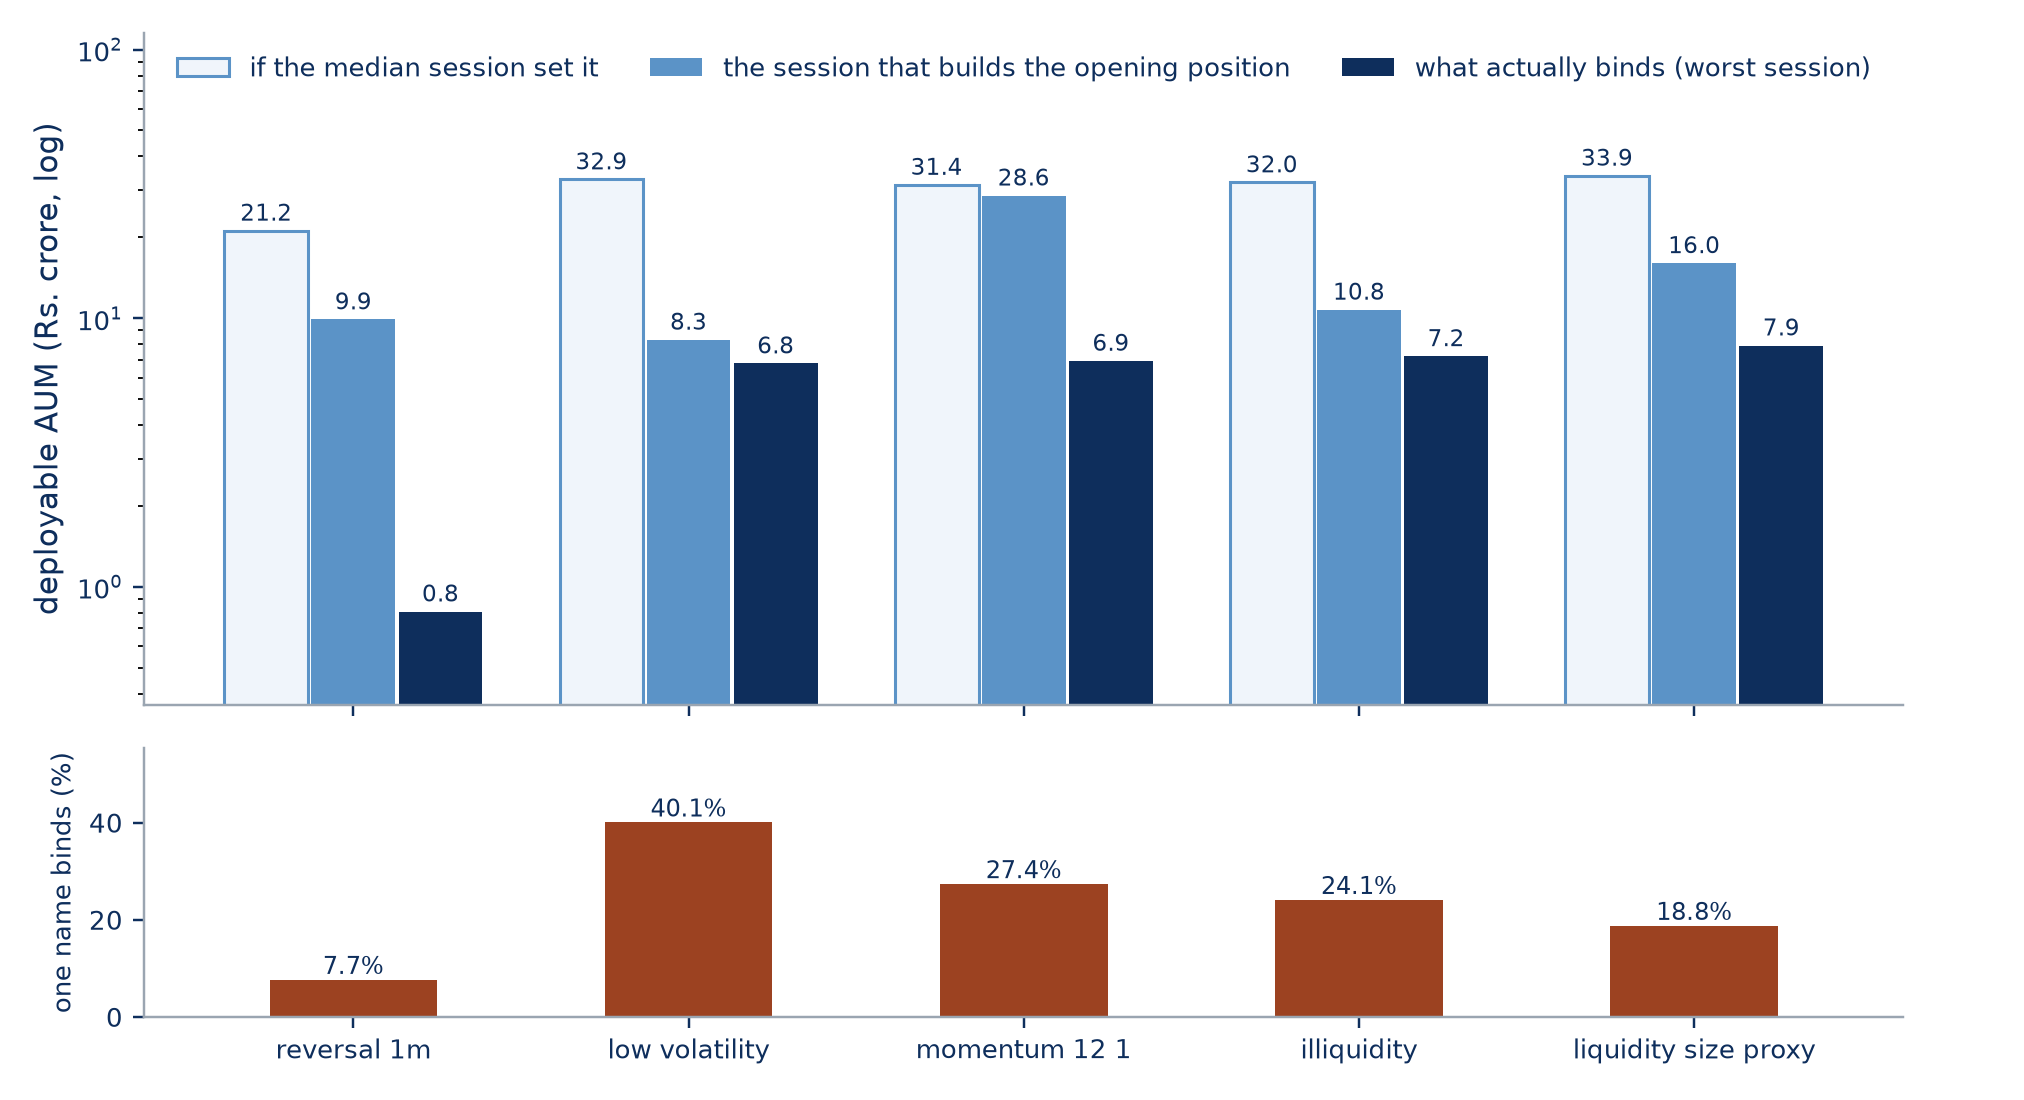
\includegraphics[width=\linewidth]{figures/fig_capacity_binding.png}
\caption{Deployment capacity in crore of rupees at a \fsParticipationLimit\% participation limit,
across \fsNFactors\ factors. \emph{Upper panel, log scale:} what capacity would be if a typical
session set it (pale), the session that builds the opening position (mid), and what actually binds
(dark). The distance between pale and dark is what a typical-session summary would have concealed.
\emph{Lower panel:} the share of sessions on which the tightest position is more than twice as
tight as the next --- that is, on which a single name is the constraint.}
\label{fig:capacitybinding}
\end{figure}

\takeaway{\textbf{The weakest position determines the capacity of the entire portfolio.} A book is
not deployable at its average liquidity --- it is deployable at the liquidity of the single worst
trade it must place, and the gap between those two readings runs from
\fsSizeProxyMedianOverBinding$\times$ to \fsReversalMedianOverBinding$\times$.}
\label{sec:capacity}

\begin{finding}
Deployment capacity is \textbf{\rupee\fsFactorBindingMin--\fsFactorBindingMax\ crore}, roughly one to
ten million US dollars. \textbf{The least liquid position the strategy holds decides it}, not the
average liquidity of its book.
\end{finding}

\paragraph{The mechanism, because the number is otherwise easy to misread.} These are equal-weighted
books. Every name in a leg carries the same weight and must therefore be traded in the same rupee
size. A strategy holding a name that turns over a tenth of what another turns over trades both
identically, and the participation constraint binds on the thinner one first. Capacity is set there,
for the whole book.

The consequence is counter-intuitive and worth stating plainly: \textbf{a strategy holding a hundred
large-capitalisation names can still be capacity-constrained by one of them.} Diversification across
many liquid names does not raise capacity if the weighting scheme forces the thinnest name to be
traded at the same size as the deepest. The \emph{one name} column reports how often this is
literally a single position.

This is not an artefact of our definition---it is the constraint a desk actually faces---but it is a
property of \emph{equal weighting} as much as of the market. The standard remedies, liquidity-tilted
weights or a liquidity screen at entry, both change the portfolio and therefore change the returns
that the capacity is a capacity \emph{for}. We measure the strategies as specified rather than
silently repairing them, and note that a capacity figure is only meaningful when paired with the
weighting scheme that produced it.

Dropping the single tightest position each session raises capacity by well under an order of
magnitude. That robustness check is what establishes these figures describe the strategy rather than
one holding; had relaxation bought tenfold, the headline would have been a statement about one name.

\subsection{Alpha decay}

\begin{figure}[t]\centering
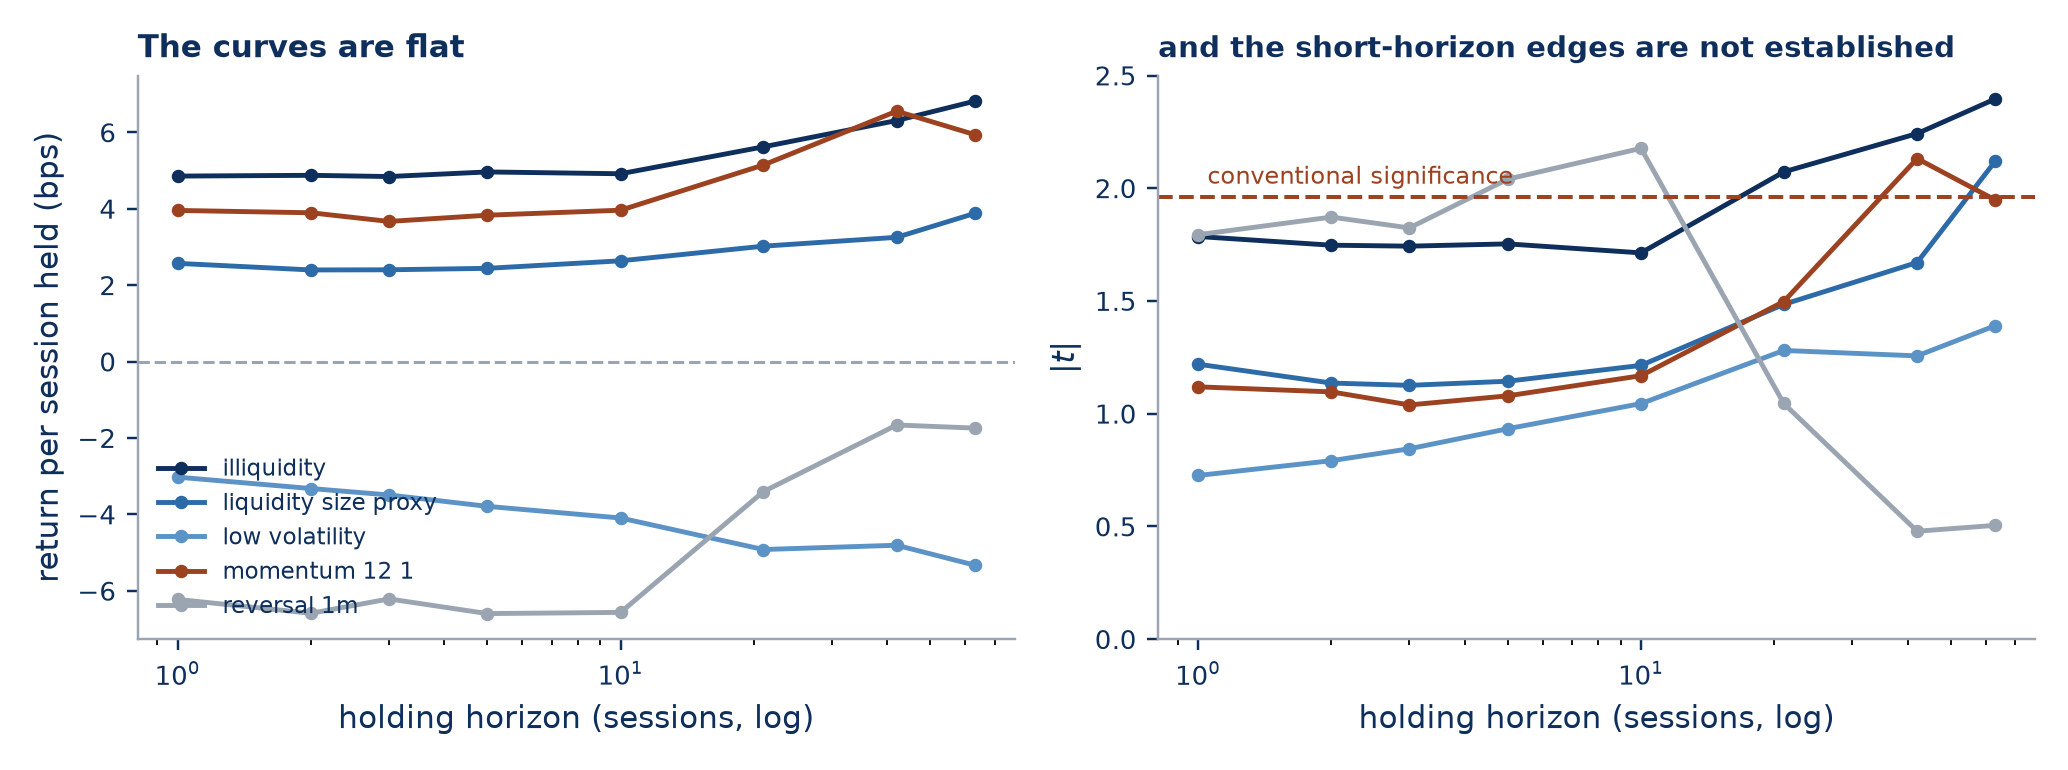
\includegraphics[width=\linewidth]{figures/fig_alpha_decay.png}
\caption{Long-short return per session held, gross of costs, across \fsNFormationDates\ formation
dates. Books are formed every session and held for $h$ sessions after a one-session execution gap,
so consecutive observations overlap; $t$-statistics divide by the number of independent holding
periods rather than the raw count, which is deliberately conservative. \emph{Left:} a decaying
edge would fall from left to right. None does. \emph{Right:} the same factors against the
conventional threshold, which no factor crosses at any horizon short enough for the question to be
about decay.}
\label{fig:decay}
\end{figure}

\begin{finding}
\textbf{\fsNFactorsWithHalfLife\ of \fsNFactors\ factors have a measurable half-life.} Every curve is
flat to gently rising out to a quarter.
\end{finding}

We report this as a null about our measurement rather than as a finding about Indian markets,
because the precondition fails. The largest $|t|$ at the shortest horizon is
\fsDecayMaxAbsTstatShortest, and the largest at any horizon in the table is \fsDecayMaxAbsTstat.
\textbf{The edges whose decay is being measured are not themselves established}, and a decay
half-life is only a meaningful quantity for a signal that had an edge to lose. Reporting one for a
factor that never made money would be a category error dressed as a measurement.

Two factors carry the wrong sign for their names, which is itself informative about the window.
\texttt{reversal\_1m} loses money, so at a one-month horizon this period shows \emph{continuation}
rather than reversal. \texttt{low\_volatility} loses, so high-beta names outperformed---consistent
with a window containing the COVID drawdown and the recovery that followed it, in which the names
that fell hardest rebounded hardest.

\paragraph{A research question retired rather than deferred.} This benchmark was specified to ask
whether alpha decays faster in India than in developed markets and whether retail participation
explains it. The first clause is answered: no decay was observed. The second therefore loses its
antecedent---there is nothing for retail participation to explain---and is retired. Delivery-share
data that would have supported a retail analysis is freely available and was deliberately not
collected, on the principle that the availability of data is not a reason to ask a question.

\subsection{Flow-conditional capacity}
\label{sec:flow}

\begin{finding}
Outflow-to-inflow capacity ratios lie between \fsFlowRatioMin\ and \fsFlowRatioMax\ across
\fsFlowNFactors\ factors, median \fsFlowRatioMedian, on
\fsFlowSessionsMin--\fsFlowSessionsMax\ sessions per cell. \textbf{The hypothesis is not supported.}
\end{finding}

The novel contribution this benchmark was built for was to ask whether deployable size collapses
when foreign participation reverses. India is a plausible place to look: foreign flows are large,
volatile, and widely believed to drive liquidity. A tenfold swing in capacity between inflow and
outflow regimes would be a useful and previously unquantified fact.

It is not there. The ratios are within a quarter of unity and some point the wrong way.

\paragraph{This null rests on a proxy, and we cannot separate two explanations.} No free source
serves historical daily foreign and domestic institutional \emph{cash-market} net flow. The exchange
publishes the series but its endpoint returns the current session regardless of the date requested,
which we verified against three parameter spellings; the alternative sources we tried returned error
pages or refused the request. The series we use instead is foreign-institutional activity in
\emph{equity derivatives}, and it differs from the intended series in three ways that are not small.
It is denominated in contracts rather than rupees, over a window in which regulatory lot sizes
changed. It describes derivatives rather than cash. And foreign derivatives activity is
substantially hedging against cash positions, so its sign need not track the direction of
cash-market demand at all.

\textbf{Whether capacity is genuinely stable across flow states, or the proxy is simply
uninformative about cash liquidity, is not separable with this data.} We state this beside the
result rather than in a limitations section, because it governs how the null may be read.

% -------------------------------------------------------------------------------------
\subsection{Why daily OHLCV cannot price transient impact}
\label{sec:identification}

\begin{figure}[t]\centering
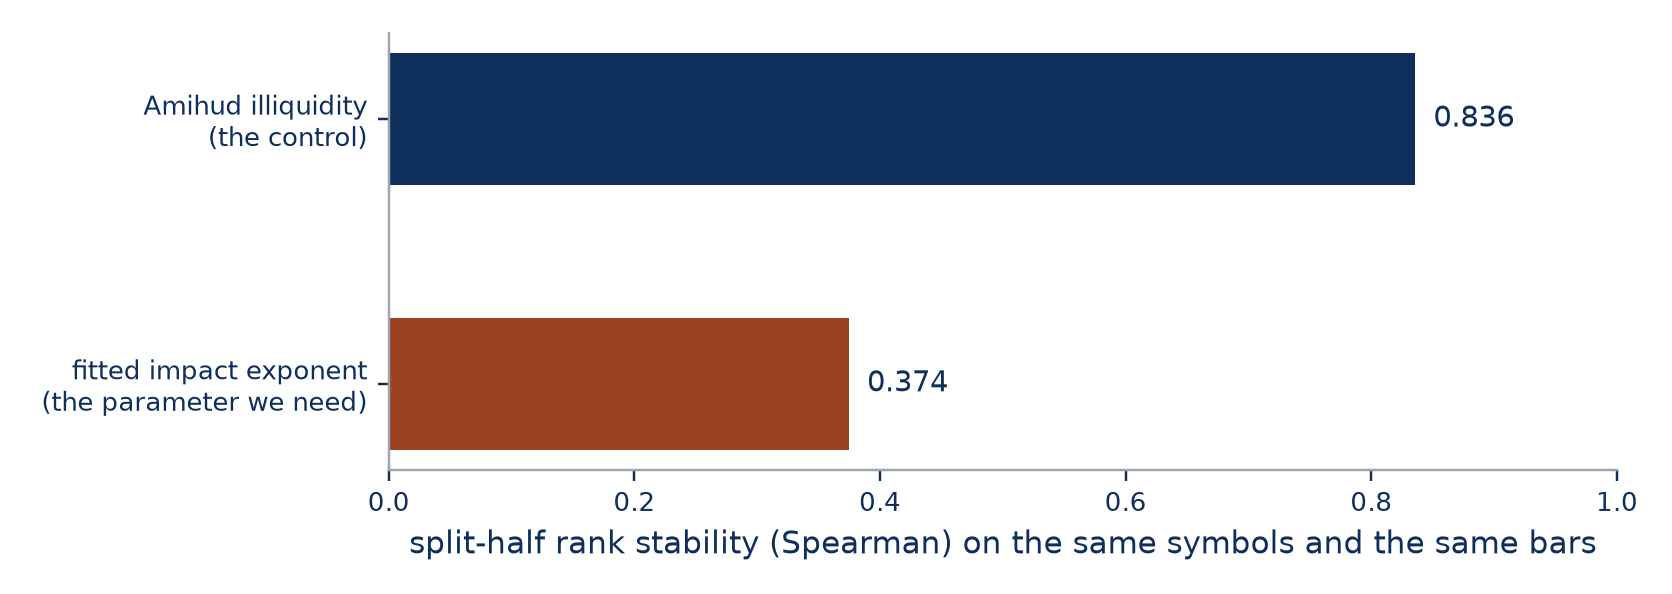
\includegraphics[width=0.86\linewidth]{figures/fig_impact_identifiability.png}
\caption{The control and the parameter, on the same daily bars, the same symbols and the same
sample split ($n=\fsAmihudN{}$). Rank stability across the split.}
\label{fig:identifiability}
\end{figure}

\takeaway{This single comparison carries the negative result. A quantity computed from exactly the
same data holds its ordering at \fsAmihudSpearman{} while the parameter a capacity study needs
reaches \fsDeltaSpearman{}. \textbf{If the data were simply too noisy, both would fail. The failure
is in the model.}}

\begin{figure}[h]\centering
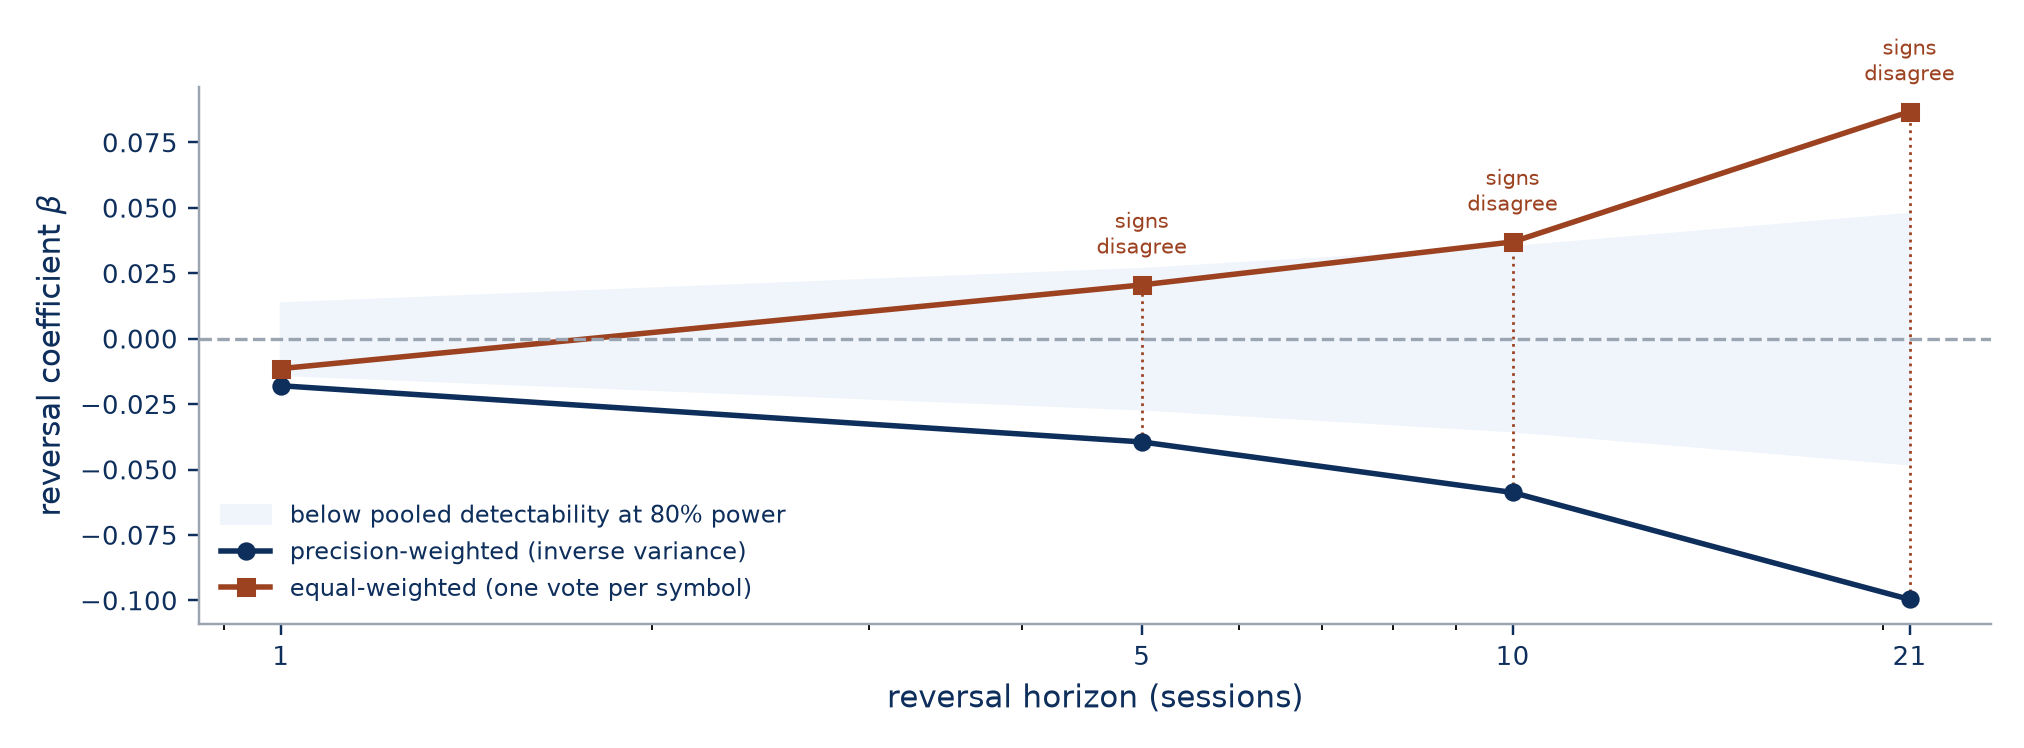
\includegraphics[width=\linewidth]{figures/fig_reversal_weighting.png}
\caption{Reversal regressions \citep{campbell1993} of the following $h$-session return on today's,
restricted to each symbol's heaviest-volume decile, $n = \fsIdentNSymbols$ symbols. Precision
weighting is inverse-variance pooling; equal weighting counts each symbol once. Both are standard
and neither is wrong. The shaded band is the effect the pooled estimator could have detected at
80\% power, so the two lines are separated by more than the data's own resolution --- the
disagreement is not a power problem, and \textbf{the sign of the coefficient is decided by the
analyst rather than by the market.}}
\label{fig:reversalweighting}
\end{figure}


A price move caused by an order is \emph{transient}: it is the cost of demanding liquidity and it is
repaid once the demand stops. A move caused by information is permanent. A negative reversal
coefficient is therefore the signature of impact, and its sign is the quantity on which any
daily-bar impact estimate depends.

\begin{finding}
\textbf{The sign depends on the weighting scheme.} Precision weighting and equal weighting are both
standard, neither is wrong, and they \textbf{disagree on sign at \fsSignDisagreements\ of
\fsHorizonsTested\ horizons}. A quantity whose sign is determined by an analyst's choice among
defensible estimators is not identified by the data.
\end{finding}

The disagreement is not a puzzle to be resolved by picking the better estimator; it is the result.
Inverse-variance pooling is correct when symbols estimate a common parameter and differ only in
noise. Equal weighting is correct when the parameter itself varies across symbols and the quantity
of interest is its population average. \textbf{Nothing in the data tells us which world we are in},
and the two answers have opposite signs. Choosing between them requires prior knowledge of exactly
the microstructure the exercise was supposed to measure.

Three further measurements agree, and one control locates the failure:

\begin{itemize}
\item \textbf{Resolution.} Temporary impact decays over minutes to hours; the finest horizon a daily
bar permits is one session. The pooled coefficient also grows monotonically more negative as the
horizon lengthens rather than decaying, which is the signature of slow mean reversion, not of a
liquidity concession being repaid.
\item \textbf{Exponent.} Fitting $|r|$ against relative traded value gives a median exponent of
\fsDeltaMedian\ against the square-root law's $0.5$, spanning \fsDeltaPTen--\fsDeltaPNinety\ across
\fsDeltaN\ symbols and explaining a median \fsFitRsquared\ of variance. Across a sample split the
per-symbol exponent correlates \fsDeltaSpearman\ with itself ($n = \fsDeltaSpearmanN$). A parameter
that does not survive its own sample split is not a parameter.
\item \textbf{Extrapolation.} A capacity study asks about \fsTargetParticipation\% participation.
Observed relative traded value has a median of \fsObservedMedianRelValue---\fsOrdersOfMagnitude\
orders of magnitude away---and only \fsSymbolDaysBelowTarget\ of \fsIdentSymbolDays\ symbol-days fall
inside the region of interest. Fitting here and applying there is not interpolation.
\item \textbf{The control.} Amihud illiquidity, computed on the same panel, correlates
\fsAmihudSpearman\ across the same split ($n = \fsAmihudN$, $p = \fsAmihudSpearmanP$). The data
supports a stable liquidity \emph{measure} while refusing to support an impact \emph{model
parameter}. \textbf{The failure is in the model, not in the data}---which is the whole reason the
control is reported.
\end{itemize}

\begin{selfreport}
\textbf{Two corrections to our own earlier reporting of this result.} An earlier version reported
that \emph{no} reversal was detected, citing the proportion of symbols with a negative coefficient
as evidence. That proportion was noise. A single symbol's daily test can detect only an effect of
\fsMdeSymbolFive\ or larger at the five-session horizon---an order of magnitude above the pooled
coefficient of \fsPooledBetaFive\ that the same data supports---so the proportion was always going to
land near half regardless of the truth. We had reported an underpowered statistic as a measurement.

Computing the detectability bound then showed that the pooled coefficient \emph{is} significantly
negative, contradicting our own earlier claim outright. The identification argument above replaced
it and is stronger. We record the sequence because the null we first reported was not the null that
survived, and a reader is entitled to know that the argument moved.
\end{selfreport}

% -------------------------------------------------------------------------------------
\subsection{The validation gap}
\label{sec:validation}

\begin{finding}
The benchmark was validated on \fsNFactors\ standard factor strategies spanning
\fsFactorSpan$\times$ in capacity, then applied to \fsCorpusN\ machine-generated strategies spanning
\fsCorpusSpan$\times$---\fsSpanRatio$\times$ wider. \textbf{Two defects lived in that gap, and the
corpus found both immediately.}
\end{finding}

Before freezing the benchmark we ran it across a corpus of strategies generated by a local language
model and previously evaluated by two companion benchmarks in the same programme. The intent was to
produce a reference corpus in which every strategy carries an audit verdict, a fragility score and a
deployment capacity; \fsCorpusAllThree\ strategies do. What it produced first was two bugs.

\paragraph{Floating-point residue counted as trading.} A strategy holding a hundred names at equal
weight and never rebalancing produces weight changes of order $10^{-18}$ from recomputing an
unchanged number. Dividing a participation limit by that residue reported its capacity as $10^{23}$
crore. The remedy is the tolerance $\varepsilon$ defined earlier.

\paragraph{The summary statistic discarded the binding constraint.} Capacity was reported as the
\emph{median} session. For a near-static book that is close to meaningless: almost every session has
near-zero rebalancing turnover, so the one tightly constrained session that builds the position was
drowned by a thousand that barely trade. The remedy is the minimum over sessions.

A subtlety worth recording, because we diagnosed it wrongly at first. We initially believed the
formula never counted the acquisition of the opening position. It did---a strategy's first session
enters at full weight from zero. \textbf{The defect was that the summary statistic discarded it},
which is a different error and took a direct check to see. Using the median would overstate the
typical corpus strategy by \fsCorpusMedianOverBinding$\times$, and entry is the binding session for
only \fsEntryBindsCount\ of \fsCorpusN\ strategies (\fsEntryBindsShare\%)---so the median was
concealing considerably more than the entry constraint alone.

Neither defect was reachable from the validation set. All five factor strategies rebalance
substantially every session, so none ever produced a near-zero traded fraction, and for all five the
median and the minimum differ by a factor small enough to look like a modelling choice rather than a
bug.

\paragraph{The corrections moved every published number down.} Capacity figures fell by between a
factor of four and a factor of twenty-six. We record the direction because it bears on whether this
counts as tuning: adapting a benchmark to flatter its subject would not systematically reduce the
results it reports. Repairing an objective omission in a definition is not the same act as adjusting
a threshold until a result improves, and the sign of the change is the cheapest available evidence
of which one happened.

We state the obvious objection rather than leave it to the reader to raise. \emph{Both defects were
found by data the benchmark was about to be applied to, and repaired before it was frozen}---the
corrections are, in the literal sense, post-hoc. Our argument that they are repairs and not tuning
rests on three things: each defect is demonstrable without reference to any result, in one case as
a dimensional absurdity and in the other as a statistic that provably omits a constraint the
definition already contained; the ordering was fixed in advance, so the corpus run was scheduled
before the freeze rather than reached for after a disappointing number; and every correction moved
every published figure downward. None of that is proof, and a reader is entitled to weigh it
themselves. We report it here, in the result, rather than in a list of caveats, because the
alternative---discovering the defects after publication, or not at all---is the outcome this
ordering exists to prevent, and a paper that buried the episode would be recommending a process it
declined to display.

\begin{finding}
The general form: \textbf{a benchmark's soundness cannot be established on the population that
motivated it.} Defects concentrate in the tails of the population a benchmark is applied to, and a
validation set assembled from familiar, well-behaved strategies has no tails.
\end{finding}

We have adopted the resulting ordering as standing process for every benchmark in this programme:
\textbf{build, validate on standard strategies, apply to the reference corpus, freeze, write up}.
The corpus run precedes the freeze and the paper. Had the original ordering held, this paper would
have shipped a capacity table containing $10^{23}$ crore.

% =====================================================================================
\section{Does any of this depend on who wrote the strategies?}
\label{sec:generators}

Every capacity figure above was measured on strategies written by one local seven-billion-parameter
model. The objection a referee reaches for first is that this measures that model rather than
machine-written strategies in general, and it is a fair objection: nothing in the preceding sections
distinguishes the two.

We therefore issued the identical frozen task specification to \fsGvArms{} frontier models through
their consumer interfaces, \fsGvRequestsPerArm{} independent requests of five strategies each, and
passed all \fsGvTotal{} through this benchmark with no parameter altered and no line of measurement
code added. The design, the hypotheses and the predicted directions were pre-registered before any
strategy was generated. Full results, including the measurements that belong to the other two
benchmarks, are in the study's own report; what follows is the part that bears on capacity.

\begin{figure}[t]\centering
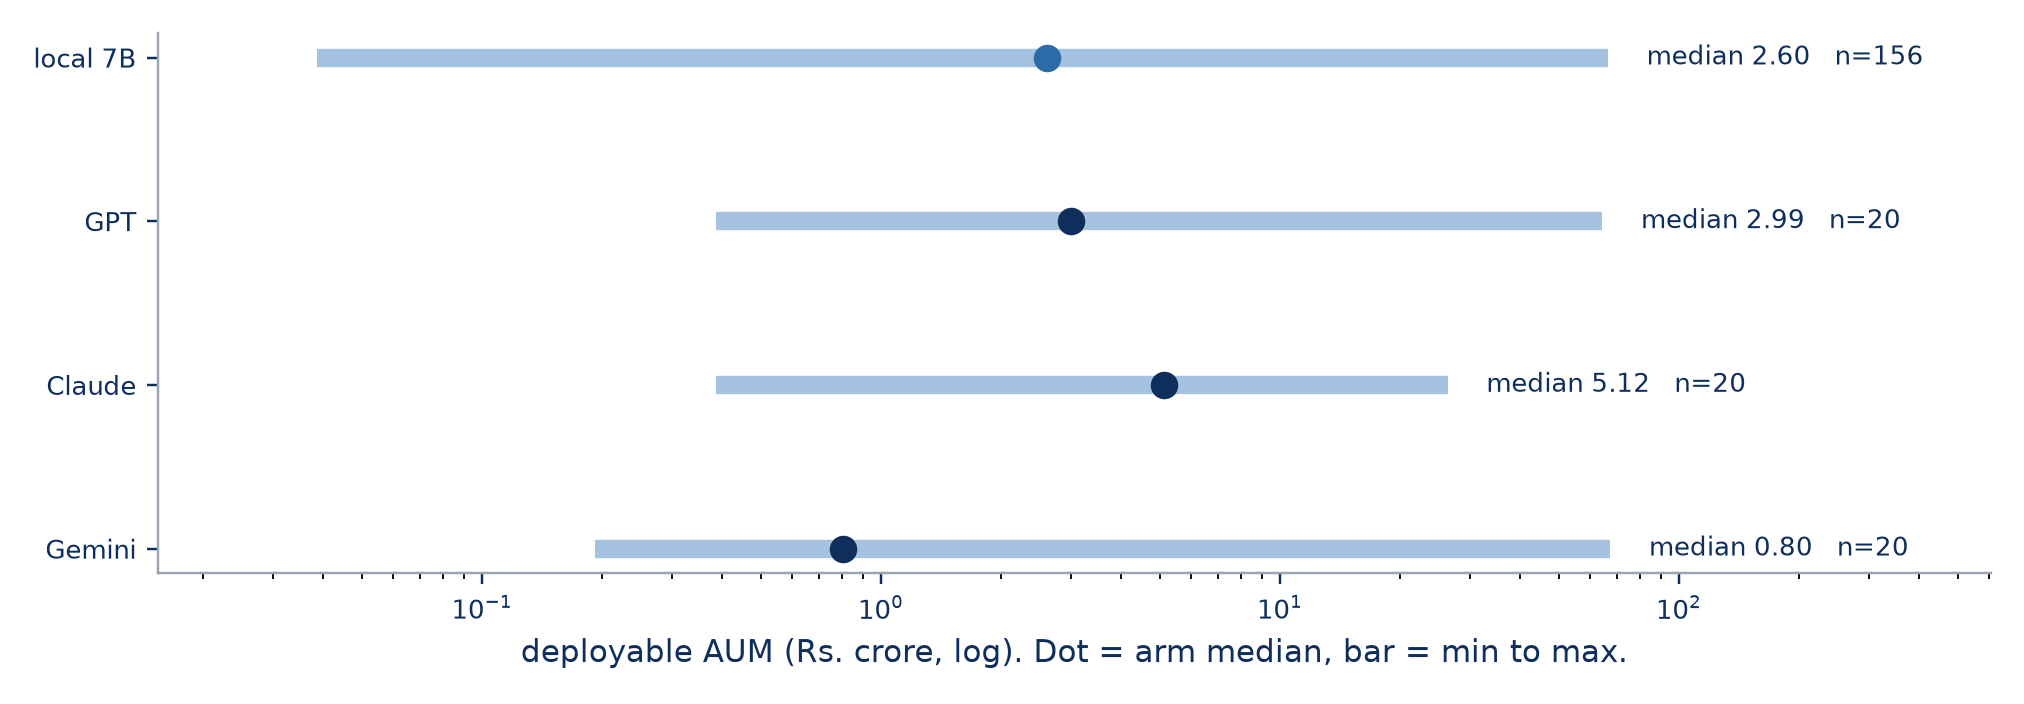
\includegraphics[width=\linewidth]{figures/fig_capacity_by_generator.png}
\caption{Constraint-based deployment capacity by generator, log scale. The dot is the arm median
and the bar is its full range. The local corpus is \fsCorpusN{} strategies; each frontier arm is
twenty. \textbf{The medians move --- one of them outside the pre-registered bound --- while every
arm spans one to two orders of magnitude internally.} The second fact is the more important one:
the spread within any single generator is wider than the gap between generators.}
\label{fig:capacitybygenerator}
\end{figure}


\paragraph{The pre-registered prediction failed on one arm of three.} We predicted that median
deployment capacity would fall within a factor of two of the local corpus for every generator, on
the reasoning that capacity is set by the traded value of Indian large caps and by the
participation limit, neither of which knows who wrote the code. Two arms are consistent with that:
GPT at \fsGvGptCapRatio{}$\times$ and Claude at \fsGvClaudeCapRatio{}$\times$. Claude clears the
stated bound by a margin far smaller than the sampling error of a twenty-strategy median, and we
report it as not clearly failing rather than as passing. Gemini Pro is
\fsGvGeminiCapRatio{}$\times$ --- outside the bound, and in the opposite direction from the one the
bound was written to catch.

\paragraph{The flow-conditional null holds too.} Section~\ref{sec:flow} reported that deployable
capital does not collapse when foreign investors withdraw --- a prediction we made and then
falsified on five factor strategies. Sixty machine-written strategies agree. The ratio of outflow
capacity to inflow capacity has a median of \fsGvGptFlowMedian{} on the GPT arm,
\fsGvClaudeFlowMedian{} on Claude and \fsGvGeminiFlowMedian{} on Gemini, against
\fsFlowRatioMedian{} for the factors. No arm's median falls below
\fsGvClaudeFlowMedian{}. Per-strategy ranges are
\fsGvGptFlowMin{}--\fsGvGptFlowMax{} on the GPT arm,
\fsGvClaudeFlowMin{}--\fsGvClaudeFlowMax{} on Claude and
\fsGvGeminiFlowMin{}--\fsGvGeminiFlowMax{} on Gemini, so not one of the
\fsGvTotal{} strategies loses even half its deployable size when flows reverse. A population that
spans two orders of magnitude in
capacity therefore reproduces a null established on one that spans less than ten times, which is
the strongest evidence this benchmark has that the flow-conditional result is a property of Indian
market liquidity rather than of the five strategies it was first measured on.

\paragraph{What we do not claim.} We have not investigated why. An account of Gemini's narrower
books would be constructed after seeing the result it explains, and would be exploratory in the
precise sense this laboratory exists to police. We state the measurement and stop.

\paragraph{What it means for this paper.} Capacity is \emph{not} generator-invariant, and any
reading of Section~\ref{sec:capacity} as a statement about machine-written strategies in general is
unsupported by this evidence. The figures in this paper describe the strategies this paper measured.
That is a narrower claim than we expected to be making, and it is the claim the data supports.

\paragraph{What survives, and is strengthened.} The \emph{mechanism} is unchanged across all four
populations: capacity is set by the least liquid name a strategy insists on trading, the span within
each arm is one to two orders of magnitude, and the frontier arms span
\fsGvGeminiCapSpan{}$\times$ at the widest against \fsCorpusSpan{}$\times$ locally. The validation
gap of Section~\ref{sec:validation} therefore recurs with more force than it was first reported
with: a benchmark validated on five factor strategies spanning under ten times was, on this
evidence, being validated on a population narrower than any generator produces.

\section{Design flaws, mistakes, and things that did not work}
\label{sec:flaws}

A benchmark that reports only its successes is not measuring anything. Everything below is a defect
in our own apparatus, a capability we withdrew, or a result that failed.

\begin{table}[h]\centering\small
\caption{Defects, withdrawals and nulls, with what each cost.}
\label{tab:flaws}
\begin{tabular}{p{0.27\linewidth}p{0.43\linewidth}p{0.22\linewidth}}
\toprule
\thead{Defect, withdrawal or null} & \thead{What it cost} & \thead{Where} \\
\midrule
Floating-point residue counted as trading &
A strategy recomputing an unchanged weight produces differences of order $10^{-18}$; dividing a
participation limit by that residue produced absurd capacities. Found only when the machine corpus
was run. & \S\ref{sec:validation} \\
\midrule
The headline statistic discarded the binding constraint &
Reporting a median session rather than the worst one overstated capacity by up to
\fsReversalMedianOverBinding$\times$. A strategy must be executable on \emph{every} rebalance. &
\S\ref{sec:validation} \\
\midrule
The price panel was truncated &
A loader discarded the warm-up rows a lookback strategy needs on its first session. Recorded as a
correction rather than treated as invalidating the published figures. & corrections log \\
\midrule
The ML impact model was withdrawn &
Originally specified here. It would have been trained to predict a quantity the data cannot
identify, and benchmarked against an equally unidentified baseline --- a comparison between two
artefacts. Deleted rather than shipped. & \S\ref{sec:identification} \\
\midrule
Value and quality factors are absent &
Both need company fundamentals this repository does not hold and could not buy at a zero budget.
The zoo is price-and-volume only, and every comparison against published factor results must be
read knowing the two most fundamentals-dependent families are missing. & \S\ref{sec:zoo} \\
\midrule
The impact coefficient stays uncalibrated, permanently &
Not a to-do. \S\ref{sec:identification} is the measurement showing it cannot be calibrated from
this data, so the cost model carries it as a stated engineering assumption forever. &
\S\ref{sec:identification} \\
\bottomrule
\end{tabular}
\end{table}

\subsection{Results that failed}

\begin{itemize}
\item \textbf{No factor has a measurable decay half-life}: \fsNFactorsWithHalfLife{} of
  \fsNFactors{}. None is statistically established even at the shortest horizon
  (largest $|t|$ = \fsDecayMaxAbsTstatShortest{}), so the precondition for a decay study fails.
  This was one of the project's three research questions.
\item \textbf{Capacity does not collapse under foreign outflows}, the effect this benchmark was
  designed to detect.
\item \textbf{Daily bars cannot price transient impact}, which was the original form of the
  headline question.
\item \textbf{Validating on standard factors was insufficient}, which we found only by doing the
  thing that exposed it.
\end{itemize}

\begin{finding}
Three of this paper's four original research questions returned nulls, and the fourth --- capacity
--- survives only because it was narrowed to a claim the data supports. \textbf{We report the
narrowing in the results rather than presenting the smaller claim as though it had always been the
plan.}
\end{finding}

% =====================================================================================
\section{Threats to validity}
\label{sec:threats}

\begin{enumerate}
\item \textbf{The flow proxy.} The flow-conditional null rests on derivatives activity rather than
cash-market flow. This is the threat we would attack first, and it is stated in the abstract and in
the result rather than only here.

\item \textbf{Capacity is an extreme-value statistic.} The headline is a minimum over roughly twelve
hundred sessions and is therefore sensitive to any one of them. We report the fifth percentile and a
drop-the-tightest-name variant alongside it, but a minimum is a minimum and should be read as one.

\item \textbf{The factor zoo is incomplete.} Value and quality are absent for want of fundamentals,
which weakens any comparison against published factor results and means the zoo over-represents
liquidity-driven signals.

\item \textbf{Decay is measured on edges that are not established.} With no factor significant at
the shortest horizon, the decay curves describe the decay of quantities that may be zero. A flat
curve through zero is not evidence of persistence.

\item \textbf{Returns are gross of costs.} Indian transaction costs are large enough to reverse the
sign of a small edge, and every decay figure here would fall under them.

\item \textbf{Equal weighting drives the capacity result.} The finding that the least liquid
position binds is a joint property of the market and of the weighting scheme. A different scheme
would give different capacities for the same signals.

\item \textbf{One market, one window.} 2020--2024 in Indian equities contains one pandemic
drawdown and one recovery. Every negative result here may be a property of that window.

\item \textbf{Intraday data would change the identification result.} We established that no free
source reaches this window at intraday resolution, and that commercially available sources at a
retail price point reach only part of it. With minute bars the extrapolation gap closes and the
transience test can be run at the scale impact actually operates. Our claim is about daily bars, not
about the phenomenon.
\end{enumerate}

% =====================================================================================
\section{What this tells us about AI-driven research}
\label{sec:meaning}

Three claims, at three scopes, kept separate --- the same discipline papers 1 and 2 apply, because
the three papers must be readable as one argument.

\paragraph{Generator-independent \tagindep} The \emph{mechanism} that sets capacity, the
flow-conditional null, and the identification failure are all properties of the market rather than
of the code put through it. The identification result does not involve a strategy at all. These
are the claims that license the benchmark being used by other people.

\paragraph{Generator-specific \taglocal} The capacity \emph{levels} are not
generator-invariant. \S\ref{sec:generators} falsified our own pre-registered prediction on one arm
of three, and the honest reading is that the figures in \S\ref{sec:capacity} describe the
strategies this paper measured rather than machine-written strategies in general. That is narrower
than we expected to be claiming.

\paragraph{Method-independent \tagmethod} The validation gap is not about language models at all.
A benchmark validated on a narrow, familiar population missed defects that a broad one exposed
immediately, and the generality of that has nothing to do with what wrote the strategies --- only
with how much of the input space the validation set covered.

\begin{finding}
Paper 1 found that a better generator writes better code without producing better evidence. Paper
2 found that it does not write more robust strategies either. This paper completes the pattern
from the other direction: \textbf{the constraint that decides how much money a strategy can absorb is
set by market liquidity, and no amount of generator capability moves it.} Across three papers,
capability moved the code and did not move the evidence.
\end{finding}

% =====================================================================================
\section{The FlowState benchmark}
\label{sec:release}

Frozen and released at \repo:

\begin{itemize}
\item \textbf{The liquidity universe.} \fsNSymbols{} symbols and
  \fsNInvestableSymbolDays{} investable symbol-days over 2020--2024, rules-based and
  survivorship-free, with a holdout year that was never opened.
\item \textbf{The capacity definition}, with its trailing-volume convention, its minimum over
  sessions, and the tolerance $\varepsilon$ that the machine corpus forced us to add.
\item \textbf{The factor zoo}, price-and-volume only, with the two families we could not build
  named rather than quietly omitted.
\item \textbf{The identification suite} --- four diagnostics, each with a detectability bound, and
  the Amihud control that locates the failure in the model rather than the data. This is shipped
  as an artefact because it is the result other researchers are most likely to want to contest.
\item \textbf{The reference corpus.} \fsCorpusAllThree{} strategies carrying an audit verdict, a
  fragility score and a deployment capacity, measured on one universe under one cost model.
\item \textbf{Every number}, regenerable from \texttt{data/raw/} by documented commands. If this
  paper and the repository disagree, the repository is right.
\end{itemize}

% =====================================================================================
\section{The companion benchmarks}
\label{sec:companions}

This benchmark is one of three built on a shared point-in-time universe, a shared Indian
transaction-cost model and a shared backtest engine, released from a single repository. A
strategy can therefore carry an audit verdict, a fragility score and a deployment capacity
measured on the same data under the same assumptions, which is what makes the
cross-benchmark statements in this paper possible.

\begin{itemize}
\item \textbf{AlphaAudit} --- whether a generated strategy is real, or an artifact of leakage and multiple testing. It supplies the strategy corpus the other two measure.\\
\href{https://github.com/Ashwin-aadi/Trivijaya-Quant-Research/blob/main/papers/pdf/alphaaudit.pdf}%
{\texttt{papers/pdf/alphaaudit.pdf}} \quad$\cdot$\quad
\href{https://github.com/Ashwin-aadi/Trivijaya-Quant-Research/tree/main/benchmarks/alphaaudit}%
{\texttt{benchmarks/alphaaudit}}

\item \textbf{RegimeStress} --- when a surviving strategy breaks, measured across counterfactual regime paths. It supplies the fragility scores and the duplicate criterion.\\
\href{https://github.com/Ashwin-aadi/Trivijaya-Quant-Research/blob/main/papers/pdf/regimestress.pdf}%
{\texttt{papers/pdf/regimestress.pdf}} \quad$\cdot$\quad
\href{https://github.com/Ashwin-aadi/Trivijaya-Quant-Research/tree/main/benchmarks/regimestress}%
{\texttt{benchmarks/regimestress}}
\item \textbf{Generator validation} --- the study of Section~\ref{sec:generators}:
the identical frozen task specification issued to three frontier models and passed
through all three benchmarks unchanged, with its pre-registration, its falsified
hypotheses and its full results.\\
\href{https://github.com/Ashwin-aadi/Trivijaya-Quant-Research/tree/main/benchmarks/generator_validation}%
{\texttt{benchmarks/generator\_validation}}
\end{itemize}

The three were designed to be read in order --- is it real, when does it break, how much
can it take --- and each answers a question the previous one raises. Every artifact,
correction log and evaluation protocol is in the repository:
\href{https://github.com/Ashwin-aadi/Trivijaya-Quant-Research}{\texttt{github.com/Ashwin-aadi/Trivijaya-Quant-Research}}.

\section{Conclusion}

FlowState reports what daily bars can support and declines what they cannot. Deployment capacity for
standard price-and-volume factors on an Indian liquidity universe is
\rupee\fsFactorBindingMin--\fsFactorBindingMax\ crore, set in every case by the least liquid position
each strategy holds rather than by the average depth of its book. No factor's edge decays measurably
within a quarter, and none is established at the shortest horizon. Deployable size does not collapse
when foreign participation reverses, though that null is conditional on a proxy we would rather not
have needed.

The result we expect to outlast the others is the one about instruments rather than about markets.
Within the estimators and information daily OHLCV affords, a transient-impact coefficient is not
identified---the obstruction is not statistical precision, but that two equally defensible estimators
disagree about its sign and the data cannot arbitrate. A great many
published backtests price market impact from daily data. This is a measurement of what that
assumption is worth, and it comes with a control showing that the same data supports a stable
liquidity measure perfectly well.

\textbf{FlowState is intended as benchmark infrastructure rather than a completed scientific
result.} It is frozen, versioned, and reproducible from raw data by a documented command sequence,
so that future strategy generators, future capacity definitions and future impact estimators can be
evaluated against the same protocol and progress can be measured against a common standard. The
corpus it now carries---\fsCorpusAllThree\ strategies with an audit verdict, a fragility score and a
deployment capacity apiece---exists to make the next comparison possible.

\subsection*{Where this leaves us}
\addcontentsline{toc}{subsection}{Where this leaves us}

This paper closes the sequence the programme set out to build. A trading idea now passes through
three questions in order --- \emph{is it real}, \emph{when does it break}, \emph{how much can it
take} --- and \fsCorpusAllThree{} machine-written strategies carry an answer to all three, on one
universe, one cost model and one backtest engine.

\begin{finding}
The programme asked whether making the AI better makes the \emph{research} better. Across three
papers the answer is consistent and narrow. \textbf{Capability moved the code and did not move the
evidence.} Frontier models took executability from \pgmLocalTrade\% to complete and left
out-of-sample performance, deflation and fragility where they were. No scaffolded generation method
beat plain prompting at matched compute. And the constraint this paper measures --- how much money a
strategy can absorb --- is a property of the market's liquidity, not of who wrote the strategy.
\end{finding}

What we would not claim is that this settles anything about AI-driven research in general. It is one
market, one window, one apparatus, with the confounds each paper names. What the three papers do
provide is the apparatus itself, frozen and public, so that the claims can be contested with
measurements rather than opinions --- including the several places where our own instruments turned
out to be the thing that failed.

% =====================================================================================
\begin{thebibliography}{9}
\bibitem[Almgren et al.(2005)]{almgren2005} Almgren, R., Thum, C., Hauptmann, E., \& Li, H. (2005).
Direct estimation of equity market impact. \emph{Risk}, 18(7), 58--62.
\bibitem[Amihud(2002)]{amihud2002} Amihud, Y. (2002). Illiquidity and stock returns: cross-section
and time-series effects. \emph{Journal of Financial Markets}, 5(1), 31--56.
\bibitem[Campbell et al.(1993)]{campbell1993} Campbell, J., Grossman, S., \& Wang, J. (1993).
Trading volume and serial correlation in stock returns. \emph{Quarterly Journal of Economics},
108(4), 905--939.
\bibitem[Jegadeesh \& Titman(1993)]{jegadeesh1993} Jegadeesh, N., \& Titman, S. (1993). Returns to
buying winners and selling losers: implications for stock market efficiency. \emph{Journal of
Finance}, 48(1), 65--91.
\bibitem[Novy-Marx \& Velikov(2016)]{novy2016} Novy-Marx, R., \& Velikov, M. (2016). A taxonomy of
anomalies and their trading costs. \emph{Review of Financial Studies}, 29(1), 104--147.
\bibitem[L\'opez de Prado(2018)]{lopez2018} L\'opez de Prado, M. (2018). \emph{Advances in Financial
Machine Learning}. Wiley.
\end{thebibliography}

\end{document}
